\documentclass[]{book}
\usepackage{lmodern}
\usepackage{amssymb,amsmath}
\usepackage{ifxetex,ifluatex}
\usepackage{fixltx2e} % provides \textsubscript
\ifnum 0\ifxetex 1\fi\ifluatex 1\fi=0 % if pdftex
  \usepackage[T1]{fontenc}
  \usepackage[utf8]{inputenc}
\else % if luatex or xelatex
  \ifxetex
    \usepackage{mathspec}
  \else
    \usepackage{fontspec}
  \fi
  \defaultfontfeatures{Ligatures=TeX,Scale=MatchLowercase}
\fi
% use upquote if available, for straight quotes in verbatim environments
\IfFileExists{upquote.sty}{\usepackage{upquote}}{}
% use microtype if available
\IfFileExists{microtype.sty}{%
\usepackage{microtype}
\UseMicrotypeSet[protrusion]{basicmath} % disable protrusion for tt fonts
}{}
\usepackage{hyperref}
\hypersetup{unicode=true,
            pdftitle={Metody przetwarzania i analizy danych w R},
            pdfauthor={Łukasz Wawrowski},
            pdfborder={0 0 0},
            breaklinks=true}
\urlstyle{same}  % don't use monospace font for urls
\usepackage{natbib}
\bibliographystyle{plainnat}
\usepackage{color}
\usepackage{fancyvrb}
\newcommand{\VerbBar}{|}
\newcommand{\VERB}{\Verb[commandchars=\\\{\}]}
\DefineVerbatimEnvironment{Highlighting}{Verbatim}{commandchars=\\\{\}}
% Add ',fontsize=\small' for more characters per line
\usepackage{framed}
\definecolor{shadecolor}{RGB}{248,248,248}
\newenvironment{Shaded}{\begin{snugshade}}{\end{snugshade}}
\newcommand{\AlertTok}[1]{\textcolor[rgb]{0.94,0.16,0.16}{#1}}
\newcommand{\AnnotationTok}[1]{\textcolor[rgb]{0.56,0.35,0.01}{\textbf{\textit{#1}}}}
\newcommand{\AttributeTok}[1]{\textcolor[rgb]{0.77,0.63,0.00}{#1}}
\newcommand{\BaseNTok}[1]{\textcolor[rgb]{0.00,0.00,0.81}{#1}}
\newcommand{\BuiltInTok}[1]{#1}
\newcommand{\CharTok}[1]{\textcolor[rgb]{0.31,0.60,0.02}{#1}}
\newcommand{\CommentTok}[1]{\textcolor[rgb]{0.56,0.35,0.01}{\textit{#1}}}
\newcommand{\CommentVarTok}[1]{\textcolor[rgb]{0.56,0.35,0.01}{\textbf{\textit{#1}}}}
\newcommand{\ConstantTok}[1]{\textcolor[rgb]{0.00,0.00,0.00}{#1}}
\newcommand{\ControlFlowTok}[1]{\textcolor[rgb]{0.13,0.29,0.53}{\textbf{#1}}}
\newcommand{\DataTypeTok}[1]{\textcolor[rgb]{0.13,0.29,0.53}{#1}}
\newcommand{\DecValTok}[1]{\textcolor[rgb]{0.00,0.00,0.81}{#1}}
\newcommand{\DocumentationTok}[1]{\textcolor[rgb]{0.56,0.35,0.01}{\textbf{\textit{#1}}}}
\newcommand{\ErrorTok}[1]{\textcolor[rgb]{0.64,0.00,0.00}{\textbf{#1}}}
\newcommand{\ExtensionTok}[1]{#1}
\newcommand{\FloatTok}[1]{\textcolor[rgb]{0.00,0.00,0.81}{#1}}
\newcommand{\FunctionTok}[1]{\textcolor[rgb]{0.00,0.00,0.00}{#1}}
\newcommand{\ImportTok}[1]{#1}
\newcommand{\InformationTok}[1]{\textcolor[rgb]{0.56,0.35,0.01}{\textbf{\textit{#1}}}}
\newcommand{\KeywordTok}[1]{\textcolor[rgb]{0.13,0.29,0.53}{\textbf{#1}}}
\newcommand{\NormalTok}[1]{#1}
\newcommand{\OperatorTok}[1]{\textcolor[rgb]{0.81,0.36,0.00}{\textbf{#1}}}
\newcommand{\OtherTok}[1]{\textcolor[rgb]{0.56,0.35,0.01}{#1}}
\newcommand{\PreprocessorTok}[1]{\textcolor[rgb]{0.56,0.35,0.01}{\textit{#1}}}
\newcommand{\RegionMarkerTok}[1]{#1}
\newcommand{\SpecialCharTok}[1]{\textcolor[rgb]{0.00,0.00,0.00}{#1}}
\newcommand{\SpecialStringTok}[1]{\textcolor[rgb]{0.31,0.60,0.02}{#1}}
\newcommand{\StringTok}[1]{\textcolor[rgb]{0.31,0.60,0.02}{#1}}
\newcommand{\VariableTok}[1]{\textcolor[rgb]{0.00,0.00,0.00}{#1}}
\newcommand{\VerbatimStringTok}[1]{\textcolor[rgb]{0.31,0.60,0.02}{#1}}
\newcommand{\WarningTok}[1]{\textcolor[rgb]{0.56,0.35,0.01}{\textbf{\textit{#1}}}}
\usepackage{longtable,booktabs}
\usepackage{graphicx,grffile}
\makeatletter
\def\maxwidth{\ifdim\Gin@nat@width>\linewidth\linewidth\else\Gin@nat@width\fi}
\def\maxheight{\ifdim\Gin@nat@height>\textheight\textheight\else\Gin@nat@height\fi}
\makeatother
% Scale images if necessary, so that they will not overflow the page
% margins by default, and it is still possible to overwrite the defaults
% using explicit options in \includegraphics[width, height, ...]{}
\setkeys{Gin}{width=\maxwidth,height=\maxheight,keepaspectratio}
\IfFileExists{parskip.sty}{%
\usepackage{parskip}
}{% else
\setlength{\parindent}{0pt}
\setlength{\parskip}{6pt plus 2pt minus 1pt}
}
\setlength{\emergencystretch}{3em}  % prevent overfull lines
\providecommand{\tightlist}{%
  \setlength{\itemsep}{0pt}\setlength{\parskip}{0pt}}
\setcounter{secnumdepth}{5}
% Redefines (sub)paragraphs to behave more like sections
\ifx\paragraph\undefined\else
\let\oldparagraph\paragraph
\renewcommand{\paragraph}[1]{\oldparagraph{#1}\mbox{}}
\fi
\ifx\subparagraph\undefined\else
\let\oldsubparagraph\subparagraph
\renewcommand{\subparagraph}[1]{\oldsubparagraph{#1}\mbox{}}
\fi

%%% Use protect on footnotes to avoid problems with footnotes in titles
\let\rmarkdownfootnote\footnote%
\def\footnote{\protect\rmarkdownfootnote}

%%% Change title format to be more compact
\usepackage{titling}

% Create subtitle command for use in maketitle
\providecommand{\subtitle}[1]{
  \posttitle{
    \begin{center}\large#1\end{center}
    }
}

\setlength{\droptitle}{-2em}

  \title{Metody przetwarzania i analizy danych w R}
    \pretitle{\vspace{\droptitle}\centering\huge}
  \posttitle{\par}
    \author{Łukasz Wawrowski}
    \preauthor{\centering\large\emph}
  \postauthor{\par}
    \date{}
    \predate{}\postdate{}
  
\usepackage{booktabs}
\usepackage{amsthm}
\makeatletter
\def\thm@space@setup{%
  \thm@preskip=8pt plus 2pt minus 4pt
  \thm@postskip=\thm@preskip
}
\makeatother

\begin{document}
\maketitle

{
\setcounter{tocdepth}{1}
\tableofcontents
}
\hypertarget{literatura}{%
\chapter*{Literatura}\label{literatura}}
\addcontentsline{toc}{chapter}{Literatura}

Podstawowa:

\begin{itemize}
\tightlist
\item
  Przemysław Biecek - \href{http://pbiecek.github.io/Przewodnik/}{\emph{Przewodnik po pakiecie R}}
\item
  Marek Gągolewski - \href{http://www.gagolewski.com/publications/programowanier/}{\emph{Programowanie w języku R. Analiza danych, obliczenia, symulacje.}}
\item
  Garret Grolemund, Hadley Wickham - \href{http://r4ds.had.co.nz/}{\emph{R for Data Science}} (\href{https://helion.pl/ksiazki/jezyk-r-kompletny-zestaw-narzedzi-dla-analitykow-danych-hadley-wickham-garrett-grolemund,jezrko.htm}{polska wersja})
\end{itemize}

Dodatkowa:

\begin{itemize}
\tightlist
\item
  \href{https://github.com/mi2-warsaw/SER/blob/master/histoRia/README.md}{inne pozycje po polsku}
\item
  \href{https://bookdown.org/}{inne pozycje po angielsku}
\end{itemize}

\href{https://github.com/lwawrowski/cdv_bigdata}{Skrypty z zajęć}

\hypertarget{wprowadzenie}{%
\chapter{Wprowadzenie}\label{wprowadzenie}}

\hypertarget{narzedzie}{%
\section{Narzędzie}\label{narzedzie}}

\begin{itemize}
\tightlist
\item
  darmowe
\item
  wszechstronne
\item
  wsparcie społeczności
\item
  wersja desktopowa i serwerowa
\end{itemize}

czyli \textbf{R} - środowisko do obliczeń statystycznych i wizualizacji wyników

\begin{itemize}
\tightlist
\item
  strona projektu: \href{https://www.r-project.org/}{r-project.org}
\item
  świetne IDE: \href{https://www.rstudio.com/}{RStudio}
\item
  wersja przeglądarkowa: \href{https://rstudio.cloud/}{rstudio.cloud}
\end{itemize}

\href{https://www.business-science.io/business/2018/10/08/python-and-r.html}{R + Python}

\hypertarget{cele-analiz}{%
\section{Cele analiz}\label{cele-analiz}}

Podstawowe:

\begin{itemize}
\tightlist
\item
  wnioskowanie statystyczne - porównywanie grup
\item
  regresja - poszukiwanie związków
\item
  klasyfikacja - przyporządkowanie do grup
\item
  grupowanie - poszukiwanie grup
\item
  prognozowanie - patrzenie w przyszłość
\end{itemize}

Inne:

\begin{itemize}
\tightlist
\item
  analiza języka naturalnego
\item
  rozpoznawanie obrazów
\item
  analiza koszykowa
\item
  \ldots{}
\end{itemize}

\hypertarget{eksporacja-danych}{%
\subsection{Eksporacja danych}\label{eksporacja-danych}}

Pakiet \texttt{tidyverse}

\begin{Shaded}
\begin{Highlighting}[]
\KeywordTok{library}\NormalTok{(tidyverse)}
\end{Highlighting}
\end{Shaded}

\begin{itemize}
\tightlist
\item
  analiza częstości dla zmiennych jakościowych
\item
  analiza struktury dla zmiennych ilościowych
\end{itemize}

Case study: \href{data/wybory2018.xlsx}{Wybory 2018}

\hypertarget{testowanie-hipotez}{%
\chapter{Testowanie hipotez}\label{testowanie-hipotez}}

\href{presentations/03_testy.html}{Prezentacja}

\hypertarget{wprowadzenie-1}{%
\section{Wprowadzenie}\label{wprowadzenie-1}}

Do rozwiązania wybranych zagadnień analizy statystycznej wystarczą metody weryfikacji hipotez statystycznych. Taki proces można przedstawić w następujących krokach:

\begin{enumerate}
\def\labelenumi{\arabic{enumi}.}
\tightlist
\item
  Sformułowanie dwóch wykluczających się hipotez - zerowej \(H_0\) oraz alternatywnej \(H_1\)
\item
  Wybór odpowiedniego testu statystycznego
\item
  Określenie dopuszczalnego prawdopodobieństwo popełnienia błędu I rodzaju (czyli poziomu istotności \(\alpha\))
\item
  Podjęcie decyzji
\end{enumerate}

Wymienione powyżej nowe pojęcia zostaną wyjaśnione poniżej.

\hypertarget{hipoteza-statystyczna}{%
\section{Hipoteza statystyczna}\label{hipoteza-statystyczna}}

Przypuszczenie dotyczące własności analizowanej cechy, np. średnia w populacji jest równa 10, rozkład cechy jest normalny.

Formułuje się zawsze dwie hipotezy: hipotezę zerową (\(H_0\)) i hipotezę alternatywną (\(H_1\)). Hipoteza zerowa jest hipotezą mówiącą o równości:

\(H_0: \bar{x}=10\)

Z kolei hipoteza alternatywna zakłada coś przeciwnego:

\(H_1: \bar{x}\neq 10\)

Zamiast znaku nierówności (\(\neq\)) może się także pojawić znak mniejszości (\(<\)) lub większości (\(>\)).

\hypertarget{poziom-istotnosci-i-wartosc-p}{%
\section{Poziom istotności i wartość p}\label{poziom-istotnosci-i-wartosc-p}}

Hipotezy statystyczne weryfikuje się przy określonym poziomie istotności \(\alpha\), który wskazuje maksymalny poziom akceptowalnego błędu (najczęściej \(\alpha=0,05\)).

Większość programów statystycznych podaje w wynikach testu wartość p.~Jest to najostrzejszy poziom istotności, przy którym możemy odrzucić hipotezę \(H_0\). Jest to rozwiązanie bardzo popularne, ale nie pozbawione wad. Dokładny opis potencjalnych zagrożeń można znaleźć w \href{http://cejsh.icm.edu.pl/cejsh/element/bwmeta1.element.cejsh-e3daa053-7cf2-4eee-9192-16c48c3a7a45/c/05.pdf}{artykule}.

Generalnie jeśli \(p < \alpha\) - odrzucamy hipotezę zerową.

\hypertarget{testy-statystyczne}{%
\section{Testy statystyczne}\label{testy-statystyczne}}

W zależności od tego co chcemy weryfikować należy wybrać odpowiedni test. Tabela poniżej przedstawia dosyć wyczerpującą klasyfikację testów pobraną ze \href{https://philipppro.github.io/Statistical_tests_overview/}{strony}.

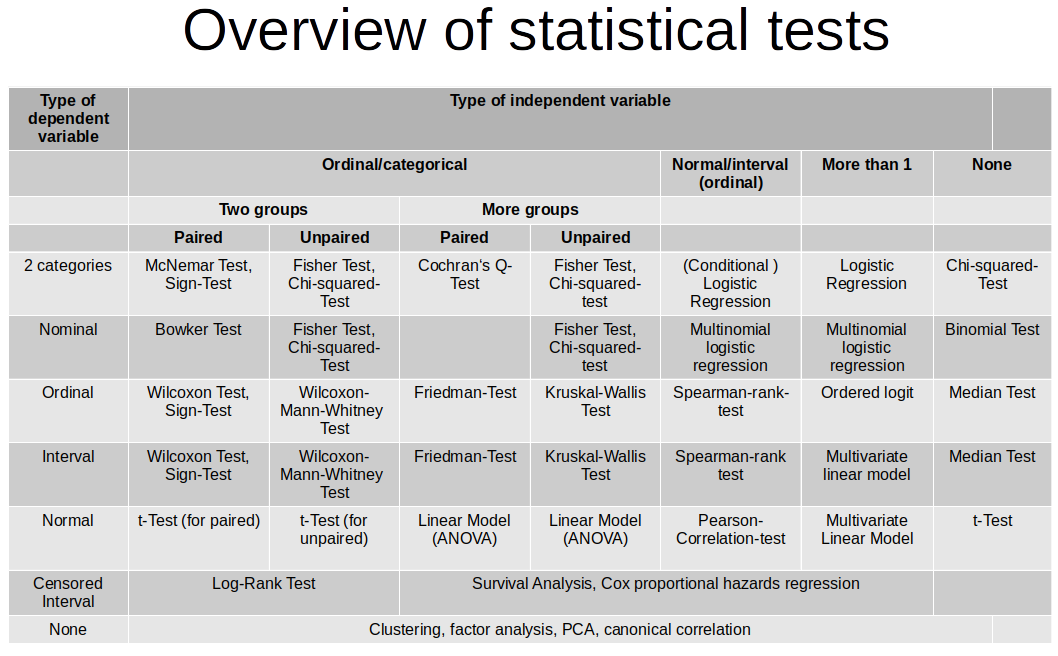
\includegraphics{img/tests.png}

\hypertarget{zbior-danych}{%
\section{Zbiór danych}\label{zbior-danych}}

Będziemy działać na zbiorze danych dotyczącym \href{data/pracownicy.xlsx}{pracowników przedsiębiorstwa}. Poniżej znajduje się opis cech znajdujących się w tym zbiorze,

\begin{itemize}
\tightlist
\item
  id - kod pracownika
\item
  plec - płeć pracownika (0 - mężczyzna, 1 - kobieta)
\item
  data\_urodz - data urodzenia
\item
  edukacja - wykształcenie (w latach nauki)
\item
  kat\_pracownika - grupa pracownicza (1 - specjalista, 2 - menedżer, 3 - konsultant)
\item
  bwynagrodzenie - bieżące wynagrodzenie
\item
  pwynagrodzenie - początkowe wynagrodzenie
\item
  staz - staż pracy (w miesiącach)
\item
  doswiadczenie - poprzednie zatrudnienie (w miesiącach)
\item
  zwiazki - przynależność do związków zawodowych (0 - nie, 1 - tak)
\item
  wiek - wiek (w latach)
\end{itemize}

\begin{Shaded}
\begin{Highlighting}[]
\KeywordTok{library}\NormalTok{(tidyverse)}
\KeywordTok{library}\NormalTok{(readxl)}

\NormalTok{pracownicy <-}\StringTok{ }\KeywordTok{read_excel}\NormalTok{(}\StringTok{"data/pracownicy.xlsx"}\NormalTok{)}
\end{Highlighting}
\end{Shaded}

\hypertarget{test-niezaleznosci}{%
\section{Test niezależności}\label{test-niezaleznosci}}

Za pomocą testu niezależności \(\chi^2\) (chi-kwadrat) można sprawdzić czy pomiędzy dwiema cechami jakościowymi występuje zależność. Układ hipotez jest następujący:

\begin{itemize}
\tightlist
\item
  \(H_0:\) zmienne są niezależne,
\item
  \(H_1:\) zmienne nie są niezależne.
\end{itemize}

W programie R test niezależności można wywołać za pomocą funkcji \texttt{chisq.test()} z pakietu \emph{stats}. Jako argument tej funkcji należy podać tablicę kontyngencji. W przypadku operowania na danych jednostkowych można ją utworzyć poprzez funkcję \texttt{table()}. Jeżeli wprowadzamy liczebności ręcznie to należy zadbać o to, żeby wprowadzony obiekt był typu \texttt{matrix}.

\textbf{Przykład}

Czy pomiędzy zmienną płeć, a zmienną przynależność do związków zawodowych istnieje zależność?

W pierwszym kroku określamy hipotezy badawcze:

\(H_0\): pomiędzy płcią a przynależnością do związków nie ma zależności

\(H_1\): pomiędzy płcią a przynależnością do związków jest zależność

oraz przyjmujemy poziom istotności - weźmy standardową wartość \(\alpha = 0,05\).

W pierwszej kolejności popatrzmy na tabelę krzyżową (kontyngencji) zawierającą liczebności poszczególnych kombinacji wariantów.

\begin{Shaded}
\begin{Highlighting}[]
\KeywordTok{table}\NormalTok{(pracownicy}\OperatorTok{$}\NormalTok{plec, pracownicy}\OperatorTok{$}\NormalTok{zwiazki)}
\end{Highlighting}
\end{Shaded}

\begin{verbatim}
##    
##       0   1
##   0 194  64
##   1 176  40
\end{verbatim}

Wartości w tej tabeli nie wskazują na liczniejszą reprezentację jednej z płci w związkach zawodowych. Zweryfikujemy zatem wskazaną hipotezę zerową z wykorzystaniem testu \(\chi^2\).

\begin{Shaded}
\begin{Highlighting}[]
\KeywordTok{chisq.test}\NormalTok{(}\KeywordTok{table}\NormalTok{(pracownicy}\OperatorTok{$}\NormalTok{plec, pracownicy}\OperatorTok{$}\NormalTok{zwiazki))}
\end{Highlighting}
\end{Shaded}

\begin{verbatim}
## 
##  Pearson's Chi-squared test with Yates' continuity correction
## 
## data:  table(pracownicy$plec, pracownicy$zwiazki)
## X-squared = 2.3592, df = 1, p-value = 0.1245
\end{verbatim}

Przy poziomie istotności \(\alpha = 0,05\), wartości p (0.1245) jest większa od wartości \(\alpha\), zatem nie ma podstaw do odrzucenia hipotezy zerowej. Można stwierdzić, że nie ma zależności pomiędzy zmiennymi płeć i przynależność do związków zawodowych.

\textbf{Przykład}

Czy pomiędzy płcią, a grupami bieżącego wynagrodzenia zdefiniowanymi przez medianę istnieje zależność?

\(H_0\): pomiędzy płcią a grupami wynagrodzenia nie ma zależności

\(H_1\): pomiędzy płcią a grupami wynagrodzenia jest zależność

W pierwszej kolejności tworzymy nową cechą zamieniając cechę \texttt{bwynagrodzenie} na zmienną jakościową posiadającą dwa warianty: poniżej mediany i powyżej mediany.

\begin{Shaded}
\begin{Highlighting}[]
\NormalTok{pracownicy <-}\StringTok{ }\NormalTok{pracownicy }\OperatorTok\StringTok{ }
\StringTok{  }\KeywordTok{mutate}\NormalTok{(}\DataTypeTok{bwyn_mediana=}\KeywordTok{cut}\NormalTok{(}\DataTypeTok{x =}\NormalTok{ bwynagrodzenie,}
                          \DataTypeTok{breaks =} \KeywordTok{c}\NormalTok{(}\KeywordTok{min}\NormalTok{(bwynagrodzenie),}
                                     \KeywordTok{median}\NormalTok{(bwynagrodzenie),}
                                     \KeywordTok{max}\NormalTok{(bwynagrodzenie)),}
                          \DataTypeTok{include.lowest =} \OtherTok{TRUE}\NormalTok{))}

\KeywordTok{table}\NormalTok{(pracownicy}\OperatorTok{$}\NormalTok{plec, pracownicy}\OperatorTok{$}\NormalTok{bwyn_mediana)}
\end{Highlighting}
\end{Shaded}

\begin{verbatim}
##    
##     [1.58e+04,2.89e+04] (2.89e+04,1.35e+05]
##   0                  73                 185
##   1                 164                  52
\end{verbatim}

W tym przypadku wygląd tablicy krzyżowej może sugerować występowanie zależności.

\begin{Shaded}
\begin{Highlighting}[]
\KeywordTok{chisq.test}\NormalTok{(}\KeywordTok{table}\NormalTok{(pracownicy}\OperatorTok{$}\NormalTok{plec, pracownicy}\OperatorTok{$}\NormalTok{bwyn_mediana))}
\end{Highlighting}
\end{Shaded}

\begin{verbatim}
## 
##  Pearson's Chi-squared test with Yates' continuity correction
## 
## data:  table(pracownicy$plec, pracownicy$bwyn_mediana)
## X-squared = 104.8, df = 1, p-value < 2.2e-16
\end{verbatim}

Test \(\chi^2\) to potwierdza - mamy podstawy do odrzucenia hipotezy zerowej na korzyść hipotezy alternatywnej - istnieje zależność pomiędzy płcią, a grupami wynagrodzenia.

\hypertarget{test-proporcji}{%
\section{Test proporcji}\label{test-proporcji}}

Test proporcji pozwala odpowiedzieć na pytanie czy odsetki w jednej, dwóch lub więcej grupach różnią się od siebie istotnie. Dla jednej próby układ hipotez został przedstawiony poniżej:

\begin{itemize}
\tightlist
\item
  \(H_0: p=p_0\)
\item
  \(H_1: p \neq p_0\) lub \(H_1: p > p_0\) lub \(H_1: p < p_0\)
\end{itemize}

Układ hipotez w przypadku dwóch prób jest następujący:

\begin{itemize}
\tightlist
\item
  \(H_0: p_1=p_2\)
\item
  \(H_1: p_1 \neq p_2\) lub \(H_1: p_1 > p_2\) lub \(H_1: p_1 < p_2\)
\end{itemize}

Dla \(k\) badanych prób hipotezę zerową i alternatywną można zapisać w następująco:

\begin{itemize}
\tightlist
\item
  \(H_0: p_1=p_2=p3=...=p_k\)
\item
  \(H_1: \exists \; p_i \neq p_j\)
\end{itemize}

W takim przypadku hipoteza alternatywna oznacza, że co najmniej jeden odsetek różni się istotnie od pozostałych.

Funkcja \texttt{prop.test} z pakietu \emph{stats} umożliwia przeprowadzanie testu proporcji w programie R. Jako argumenty należy podać wektor, który zawiera licznik badanych odsetków - \texttt{x}, oraz wektor zawierający wartości mianownika - \texttt{n}. W przypadku jednej próby należy jeszcze dodać argument \texttt{p}, którego wartość oznacza weryfikowany odsetek.

\textbf{Przykład}

Wysunięto przypuszczenie, że palacze papierosów stanowią jednakowy odsetek wśród mężczyzn i kobiet. W celu sprawdzenia tej hipotezy wylosowano 500 mężczyzn i 600 kobiet. Okazało się, że wśród mężczyzn było 200 palaczy, a wśród kobiet 250.

\(H_0\): odsetek palaczy wg płci jest taki sam

\(H_1\): odsetek palaczy różni się wg płci

\begin{Shaded}
\begin{Highlighting}[]
\KeywordTok{prop.test}\NormalTok{(}\DataTypeTok{x =} \KeywordTok{c}\NormalTok{(}\DecValTok{200}\NormalTok{,}\DecValTok{250}\NormalTok{), }\DataTypeTok{n =} \KeywordTok{c}\NormalTok{(}\DecValTok{500}\NormalTok{,}\DecValTok{600}\NormalTok{))}
\end{Highlighting}
\end{Shaded}

\begin{verbatim}
## 
##  2-sample test for equality of proportions with continuity
##  correction
## 
## data:  c(200, 250) out of c(500, 600)
## X-squared = 0.24824, df = 1, p-value = 0.6183
## alternative hypothesis: two.sided
## 95 percent confidence interval:
##  -0.07680992  0.04347659
## sample estimates:
##    prop 1    prop 2 
## 0.4000000 0.4166667
\end{verbatim}

Przy poziomie istotności 0,05 nie ma podstaw do odrzucenia H0 - odsetek palaczy jest taki sam w grupach płci.

\hypertarget{testowanie-normalnosci---test-shapiro-wilka}{%
\section{Testowanie normalności - test Shapiro-Wilka}\label{testowanie-normalnosci---test-shapiro-wilka}}

Testy parametryczne z reguły wymagają spełnienia założenia o normalności rozkładu. W celu weryfikacji tego założenia należy wykorzystać jeden z testów normalności.

W celu formalnego zweryfikowania rozkładu cechy można wykorzystać test Shapiro-Wilka. Układ hipotez z tym teście jest następujący:

\begin{itemize}
\tightlist
\item
  \(H_0: F(x) = F_0(x)\) - rozkład cechy ma rozkład normalny
\item
  \(H_1: F(x) \neq F_0(x)\) - rozkład cechy nie ma rozkładu normalnego
\end{itemize}

W przeprowadzonych dotychczas symulacjach wykazano, że test Shapiro-Wilka ma największą moc spośród testów normalności, niemniej jego ograniczeniem jest maksymalna liczba obserwacji, która wynosi 5000\footnote{W przypadku liczniejszych prób można wykorzystać test Kołmogorowa-Smirnova.}.

W programie R test Shapiro-Wilka można uruchomić za pomocą funkcji \texttt{shapiro.test()} jako argument podając wektor wartości liczbowych, który chcemy zweryfikować.

\hypertarget{testowanie-normalnosci---wykres-kwantyl-kwantyl}{%
\section{Testowanie normalności - wykres kwantyl-kwantyl}\label{testowanie-normalnosci---wykres-kwantyl-kwantyl}}

Normalność rozkładu może także zostać zweryfikowana poprzez utworzenie wykresu przedstawiającego porównanie wartości oryginalnych oraz odpowiadającym im wartości pochodzących z rozkładu normalnego. Dodatkowo prowadzona jest linia regresji pomiędzy otrzymanymi wartościami. Punkty przebiegające w pobliżu tej linii oznaczają, że rozkład tej cechy jest normalny.

Na wykresie przedstawiony jest wykres kwantyl-kwantyl dla 50 wartości wylosowanych z rozkładu normalnego i z rozkładu jednostajnego.

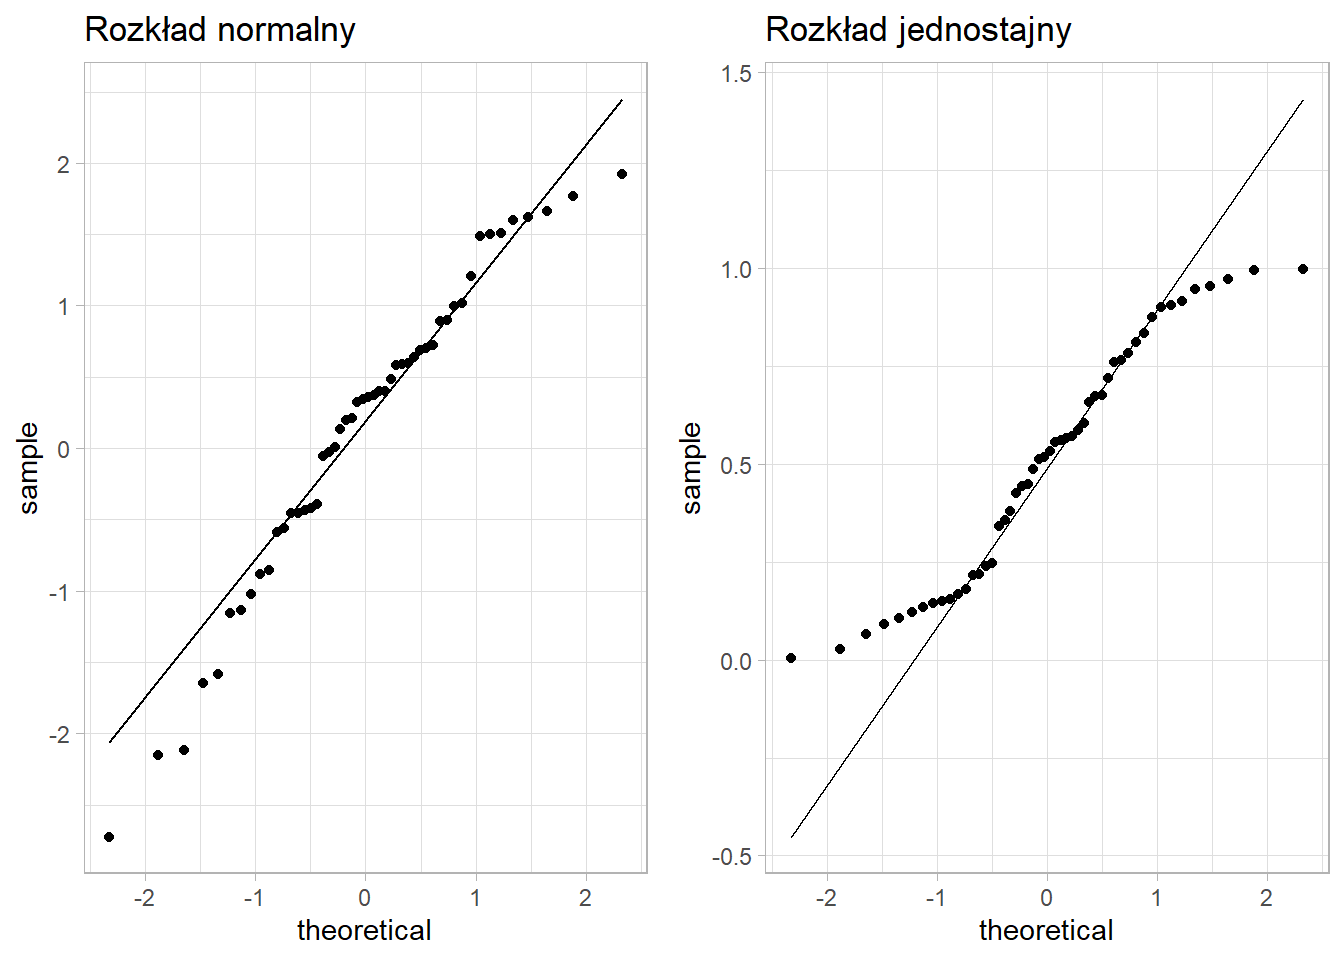
\includegraphics{Wawrowski_ADR_files/figure-latex/unnamed-chunk-9-1.pdf}

Jak można zauważyć punkty na wykresie po lewej stronie nie odbiegają znacząco od linii prostej, zatem można przypuszczać, że rozkład tej cechy jest normalny. Z kolei na wykresie po prawej stronie obserwuje się odstępstwo od rozkładu normalnego - wartości na krańcach linii są od niej oddalone.

\textbf{Przykład}

Czy cecha \emph{doświadczenie} ma rozkład normalny? Sprawdź za pomocą odpowiedniego testu oraz wykresu kwantyl-kwantyl.

\(H_0\): doświadczenie ma rozkład normalny

\(H_1\): doświadczenie nie ma rozkładu normalnego

\begin{Shaded}
\begin{Highlighting}[]
\KeywordTok{shapiro.test}\NormalTok{(pracownicy}\OperatorTok{$}\NormalTok{doswiadczenie)}
\end{Highlighting}
\end{Shaded}

\begin{verbatim}
## 
##  Shapiro-Wilk normality test
## 
## data:  pracownicy$doswiadczenie
## W = 0.8136, p-value < 2.2e-16
\end{verbatim}

Na poziomie \(\alpha = 0,05\) Odrzucamy \(H_0\) (p \textless{} \(\alpha\)) - doświadczenie nie ma rozkładu normalnego. Sprawdźmy jeszcze jak te wartości wyglądają na wykresie kwantyl-kwantyl.

\begin{Shaded}
\begin{Highlighting}[]
\KeywordTok{ggplot}\NormalTok{(pracownicy, }\KeywordTok{aes}\NormalTok{(}\DataTypeTok{sample =}\NormalTok{ doswiadczenie)) }\OperatorTok{+}
\StringTok{  }\KeywordTok{stat_qq}\NormalTok{() }\OperatorTok{+}
\StringTok{  }\KeywordTok{stat_qq_line}\NormalTok{()}
\end{Highlighting}
\end{Shaded}

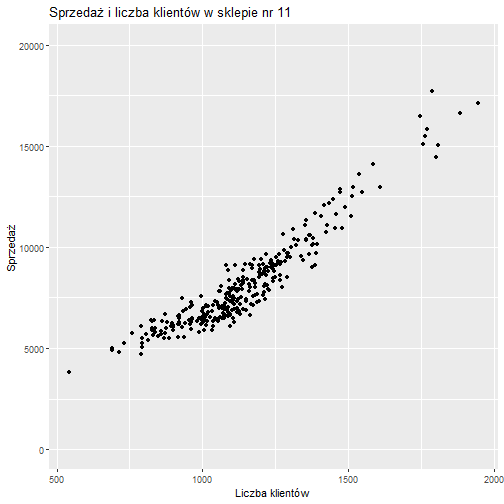
\includegraphics{Wawrowski_ADR_files/figure-latex/unnamed-chunk-11-1.pdf}

\hypertarget{testowanie-wariancji---test-bartletta}{%
\section{Testowanie wariancji - test Bartletta}\label{testowanie-wariancji---test-bartletta}}

Oprócz założenia o normalności, niektóre metody statystyczne wymagają także równości wariancji.

Jeśli chcemy sprawdzić homogeniczność wariancji w dwóch lub więcej grupach to należy skorzystać z testu Bartletta:

\begin{itemize}
\tightlist
\item
  \(H_0: s^2_1=s^2_2= s^2_3 =...=s^2_k\)
\item
  \(H_1: \exists_{i,j\in\{1,..,k\}} \; s^2_i \neq s^2_j\)
\end{itemize}

Funkcja \texttt{bartlett.test()} w programie R umożliwia zastosowanie tego testu. Argumenty do tej funkcji można przekazać na dwa sposoby. Pierwszy polega na przypisaniu do argumentu \texttt{x} wektora zawierającego wartości cechy, a do argumentu \texttt{g} wektora zawierającego identyfikatory poszczególnych grup. Drugi sposób to zadeklarowanie formuły w postaci \texttt{zmienna\_analizowa\ \textasciitilde{}\ zmienna\_grupująca} oraz podanie zbioru danych przypisanego do argumentu \texttt{data}.

\textbf{Przykład}

Sprawdźmy czy wariancje zmiennej \texttt{doświadczenie} w grupach płci są takie same.

\(H_0\): wariancje doświadczenia są takie same w grupach płci

\(H_1\): wariancje doświadczenia nie są takie same w grupach płci

Funkcję weryfikującą \(H_0\) można zapisać na dwa sposoby - wynik zawsze będzie taki sam.

\begin{Shaded}
\begin{Highlighting}[]
\KeywordTok{bartlett.test}\NormalTok{(}\DataTypeTok{x =}\NormalTok{ pracownicy}\OperatorTok{$}\NormalTok{doswiadczenie, }\DataTypeTok{g =}\NormalTok{ pracownicy}\OperatorTok{$}\NormalTok{plec)}
\end{Highlighting}
\end{Shaded}

\begin{verbatim}
## 
##  Bartlett test of homogeneity of variances
## 
## data:  pracownicy$doswiadczenie and pracownicy$plec
## Bartlett's K-squared = 4.7659, df = 1, p-value = 0.02903
\end{verbatim}

\begin{Shaded}
\begin{Highlighting}[]
\KeywordTok{bartlett.test}\NormalTok{(pracownicy}\OperatorTok{$}\NormalTok{doswiadczenie }\OperatorTok{~}\StringTok{ }\NormalTok{pracownicy}\OperatorTok{$}\NormalTok{plec)}
\end{Highlighting}
\end{Shaded}

\begin{verbatim}
## 
##  Bartlett test of homogeneity of variances
## 
## data:  pracownicy$doswiadczenie by pracownicy$plec
## Bartlett's K-squared = 4.7659, df = 1, p-value = 0.02903
\end{verbatim}

Przyjmując poziom istotności \(\alpha = 0,05\) odrzucamy hipotezę zerową stwierdzając, że wariancje różnią się w grupach płci. Z kolei dopuszczając niższy poziom istotności \(\alpha = 0,01\) podjęlibyśmy decyzję o braku podstaw do odrzucenia \(H_0\) i nieistotnej różnicy pomiędzy grupami.

\hypertarget{testowanie-srednich}{%
\section{Testowanie średnich}\label{testowanie-srednich}}

W przypadku testowania wartości przeciętnych należy wprowadzić pojęcie prób zależnych i niezależnych:

\begin{itemize}
\item
  próby zależne (paired) - analizowane są te same jednostki, ale różne cechy.
\item
  próby niezależne (unpaired) - analizowane są różne jednostki, ale ta sama cecha.
\end{itemize}

W zależności od tego czy spełnione są odpowiednie założenia dotyczące normalności cechy oraz równości wariancji należy wybrać odpowiedni test według poniższego diagramu.

\includegraphics{img/07_testy_diagram_v3.png}

\hypertarget{test-t-srednich}{%
\subsection{Test t-średnich}\label{test-t-srednich}}

Weryfikacja równości średnich może odbywać się na zasadzie porównania wartości średniej w jednej grupie z arbitralnie przyjętym poziomem lub w dwóch różnych grupach. W pierwszym przypadku rozważamy układ hipotez:

\begin{itemize}
\tightlist
\item
  \(H_0: m = m_0\)
\item
  \(H_1: m \neq m_0\) lub \(H_1: m < m_0\) lub \(H_1: m > m_0\)
\end{itemize}

natomiast w drugim przypadku hipotezy będą wyglądać następująco:

\begin{itemize}
\tightlist
\item
  \(H_0: m_1 = m_2\)
\item
  \(H_1: m_1 \neq m_2\) lub \(H_1: m_1 < m_2\) lub \(H_1: m_1 > m_2\)
\end{itemize}

Alternatywnie hipotezę zerową można zapisać jako \(m_1 - m_2 = 0\) czyli sprawdzamy czy różnica pomiędzy grupami istotnie różni się od zera.

W funkcji \texttt{t.test()} z pakietu \emph{stats} w przypadku jednej próby należy podać argument \texttt{x} czyli wektor z wartościami, które są analizowane oraz wartość, z którą tą średnią porównujemy (argument \texttt{mu}, który domyślnie jest równy 0). Dodatkowo w argumencie \texttt{alternative} wskazujemy jaką hipotezę alternatywną bierzemy pod uwagę.

Dla weryfikacji równości średniej w dwóch próbach należy dodać argument \texttt{y} z wartościami w drugiej próbie. W tym przypadku mamy także możliwość określenia czy próby są zależne (argument \texttt{paired}) lub czy wariancja w obu próbach jest taka sama (\texttt{var.equal}). Jeżeli wariancje są różne to program R przeprowadzi test t Welcha i liczba stopni swobody nie będzie liczbą całkowitą.

\hypertarget{anova}{%
\subsection{ANOVA}\label{anova}}

W przypadku większej liczby grup stosuje się jednoczynnikową analizę wariancji (ANOVA). Ta analiza wymaga spełnienia założenia o normalności rozkładu i równości wariancji w badanych grupach. Układ hipotez jest następujący:

\begin{itemize}
\tightlist
\item
  \(H_0: m_1 = m_2 = m_3 = ... = m_k\)
\item
  \(H_1: \exists_{i,j\in\{1,..,k\}} \; m_i \neq m_j\)
\end{itemize}

Za pomocą funkcji \texttt{aov()} można w R przeprowadzić jednoczynnikową analizę wariancji. Jako argument funkcji należy podać formułę przedstawiającą zależność zmiennej badanej do zmiennej grupującej wykorzystując w tym celu symbol tyldy (\texttt{\textasciitilde{}}) w następującym kontekście: \texttt{zmienna\_analizowana\ \textasciitilde{}\ zmienna\_grupująca}. Przy takim zapisie należy także w argumencie \texttt{data} podać nazwę zbioru danych.

W porównaniu do wcześniej opisanych funkcji, \texttt{aov()} nie zwraca w bezpośrednim wyniku wartości p.~Aby uzyskać tę wartość należy wynik działania tej funkcji przypisać do obiektu, a następnie na nim wywołać funkcję \texttt{summary()}.

W przypadku odrzucenia hipotezy zerowej można przeprowadzić test Tukeya w celu identyfikacji różniących się par wykorzystując funkcję \texttt{TukeyHSD()} i jako argument podając obiekt zawierający wynik ANOVA.

W sytuacji, w której założenia użycia testu parametrycznego nie są spełnione, należy skorzystać z testów nieparametrycznych. W przypadku testowania miar tendencji centralnej różnica pomiędzy testami parametrycznymi a nieparametrycznymi polega na zastąpieniu wartości średniej medianą. Z punktu widzenia obliczeń w miejsce oryginalnych wartości cechy wprowadza się rangi czyli następuje osłabienie skali pomiarowej - z ilorazowej na porządkową.

\hypertarget{test-wilcoxona}{%
\subsection{Test Wilcoxona}\label{test-wilcoxona}}

Test Wilcoxona jest nieparametryczną wersją testu t. Hipotezy w tym teście dotyczą równości rozkładów:

\begin{itemize}
\tightlist
\item
  \(H_0: F_1=F_2\)
\item
  \(H_1: F_1 \neq F_2\)
\end{itemize}

Wartość statystyki testowej będzie zależna od typu testu, natomiast w R funkcja, której należy użyć to \texttt{wilcox.test()}. Argumenty tej funkcji są takie same jak w przypadku testu t.

\hypertarget{test-kruskala-wallisa}{%
\subsection{Test Kruskala-Wallisa}\label{test-kruskala-wallisa}}

Z kolei test Kruskala-Wallisa jest nieparametrycznym odpowiednikiem ANOVA. Hipotezy są następujące:

\begin{itemize}
\tightlist
\item
  \(H_0: F_1=F_2=F_3=...=F_k\)
\item
  \(H_1: \exists_{i,j\in\{1,..,k\}} \; F_i \neq F_j\)
\end{itemize}

W programie R korzysta się z funkcji \texttt{kruskal.test()}, która przyjmuje takie same argumenty jak funkcja do metody ANOVA \texttt{aov()}. Główną różnicą jest sposób podawania wyniku testu, ponieważ w tym przypadku od razu otrzymujemy wartość p.~W przypadku odrzucenia hipotezy zerowej należy sprawdzić, które grupy różnią się między sobą. Można to zrobić za pomocą funkcji \texttt{pairwise.wilcox.test()}.

\textbf{Przykład}

Sprawdzimy czy średnie doświadczenie w grupach płci jest takie same.

\(H_0\): średnie doświadczenie w grupach płci jest takie samo

\(H_1\): średnie doświadczenie w grupach płci nie jest takie samo

W związku z tym, że badana cecha nie ma rozkładu normalnego zostanie przeprowadzony test Wilcoxona. Mamy tutaj do czynienia z testem dla prób niezależnych - badana jest jedna cecha (doświadczenie) w ramach rozłącznych grup płci.

\begin{Shaded}
\begin{Highlighting}[]
\KeywordTok{wilcox.test}\NormalTok{(pracownicy}\OperatorTok{$}\NormalTok{doswiadczenie }\OperatorTok{~}\StringTok{ }\NormalTok{pracownicy}\OperatorTok{$}\NormalTok{plec)}
\end{Highlighting}
\end{Shaded}

\begin{verbatim}
## 
##  Wilcoxon rank sum test with continuity correction
## 
## data:  pracownicy$doswiadczenie by pracownicy$plec
## W = 36295, p-value = 0.00000001372
## alternative hypothesis: true location shift is not equal to 0
\end{verbatim}

Przyjmując poziom istotności \(\alpha = 0,05\) odrzucamy \(H_0\) - średnie doświadczenie nie jest takie samo.

\textbf{Przykład}

Czy początkowe i bieżące wynagrodzenie różni się od siebie w sposób istotny?

\(H_0\): średnie początkowe i bieżące wynagrodzenie jest takie samo

\(H_1\): średnie początkowe i bieżące wynagrodzenie nie jest takie samo

W pierwszej kolejności weryfikujemy normalność rozkładu analizowanych cech.

\begin{Shaded}
\begin{Highlighting}[]
\KeywordTok{shapiro.test}\NormalTok{(pracownicy}\OperatorTok{$}\NormalTok{pwynagrodzenie)}
\end{Highlighting}
\end{Shaded}

\begin{verbatim}
## 
##  Shapiro-Wilk normality test
## 
## data:  pracownicy$pwynagrodzenie
## W = 0.71535, p-value < 2.2e-16
\end{verbatim}

\begin{Shaded}
\begin{Highlighting}[]
\KeywordTok{shapiro.test}\NormalTok{(pracownicy}\OperatorTok{$}\NormalTok{bwynagrodzenie)}
\end{Highlighting}
\end{Shaded}

\begin{verbatim}
## 
##  Shapiro-Wilk normality test
## 
## data:  pracownicy$bwynagrodzenie
## W = 0.77061, p-value < 2.2e-16
\end{verbatim}

Wynagrodzenie w tym zbiorze danych zdecydowanie nie przypomina rozkładu normalnego. W tym przypadku analizujemy próby zależne - badamy dwie różne cechy dla tych samych jednostek (obserwacji).

\begin{Shaded}
\begin{Highlighting}[]
\KeywordTok{wilcox.test}\NormalTok{(}\DataTypeTok{x =}\NormalTok{ pracownicy}\OperatorTok{$}\NormalTok{pwynagrodzenie, }
            \DataTypeTok{y =}\NormalTok{ pracownicy}\OperatorTok{$}\NormalTok{bwynagrodzenie,}
            \DataTypeTok{paired =} \OtherTok{TRUE}\NormalTok{)}
\end{Highlighting}
\end{Shaded}

\begin{verbatim}
## 
##  Wilcoxon signed rank test with continuity correction
## 
## data:  pracownicy$pwynagrodzenie and pracownicy$bwynagrodzenie
## V = 0, p-value < 2.2e-16
## alternative hypothesis: true location shift is not equal to 0
\end{verbatim}

Na podstawie podanej wartości p odrzucamy \(H_0\) - średnie początkowe i bieżące wynagrodzenie różni się od siebie istotnie statystycznie.

\textbf{Przykład}

Analogicznie można także sprawdzić czy np. doświadczenie różni się w ramach więcej niż dwóch grup - w takim przypadku rozpatrujemy głównie próby niezależne.

\(H_0\): średnie doświadczenie w grupach kategorii pracownika jest takie same

\(H_1\): średnie doświadczenie w grupach kategorii pracownika nie jest takie same - co najmniej jedna para jest różna

\begin{Shaded}
\begin{Highlighting}[]
\KeywordTok{kruskal.test}\NormalTok{(pracownicy}\OperatorTok{$}\NormalTok{doswiadczenie }\OperatorTok{~}\StringTok{ }\NormalTok{pracownicy}\OperatorTok{$}\NormalTok{kat_pracownika)}
\end{Highlighting}
\end{Shaded}

\begin{verbatim}
## 
##  Kruskal-Wallis rank sum test
## 
## data:  pracownicy$doswiadczenie by pracownicy$kat_pracownika
## Kruskal-Wallis chi-squared = 57.466, df = 2, p-value = 3.322e-13
\end{verbatim}

Przyjmując poziom istotności \(\alpha = 0,05\) odrzucamy hipotezę zerową - co najmniej jedna para kategorii pracownika różni się pod względem średniego wynagrodzenia.

\hypertarget{regresja}{%
\chapter{Regresja}\label{regresja}}

\href{presentations/04_regresja.html}{Prezentacja}

\hypertarget{wprowadzenie-2}{%
\section{Wprowadzenie}\label{wprowadzenie-2}}

Metody regresji pozwalają na analizowanie zależności przyczynowo-skutkowych oraz predycję nieznanych wartości. Korzystając z tej metody należy jednak pamiętać, że model regresji jest tylko przybliżeniem rzeczywistości.

Przykłady zastosowania regresji:

\begin{itemize}
\item
  zależność wielkości sprzedaży od wydatków na reklamę
\item
  zależność wynagrodzenia od lat doświadczenia
\end{itemize}

Na początku pracy wczytujemy biblioteki \emph{tidyverse} i \emph{readxl}.

\begin{Shaded}
\begin{Highlighting}[]
\KeywordTok{library}\NormalTok{(tidyverse)}
\KeywordTok{library}\NormalTok{(readxl)}
\end{Highlighting}
\end{Shaded}

\hypertarget{regresja-prosta}{%
\section{Regresja prosta}\label{regresja-prosta}}

Na podstawie \href{data/salary.xlsx}{danych} dotyczących informacji o doświadczeniu i wynagrodzeniu pracowników zbuduj model określający `widełki' dla potencjalnych pracowników o doświadczeniu równym 8, 10 i 11 lat.

Wczytujemy dane i sprawdzamy czy nie występują zera bądź braki danych z użyciem funkcji \texttt{summary()}.

\begin{Shaded}
\begin{Highlighting}[]
\NormalTok{salary <-}\StringTok{ }\KeywordTok{read_xlsx}\NormalTok{(}\StringTok{"data/salary.xlsx"}\NormalTok{)}

\KeywordTok{summary}\NormalTok{(salary)}
\end{Highlighting}
\end{Shaded}

\begin{verbatim}
##  YearsExperience      Salary      
##  Min.   : 1.100   Min.   : 37731  
##  1st Qu.: 3.200   1st Qu.: 56721  
##  Median : 4.700   Median : 65237  
##  Mean   : 5.313   Mean   : 76003  
##  3rd Qu.: 7.700   3rd Qu.:100545  
##  Max.   :10.500   Max.   :122391
\end{verbatim}

Następnie stworzymy wykres.

\begin{Shaded}
\begin{Highlighting}[]
\KeywordTok{plot}\NormalTok{(salary)}
\end{Highlighting}
\end{Shaded}

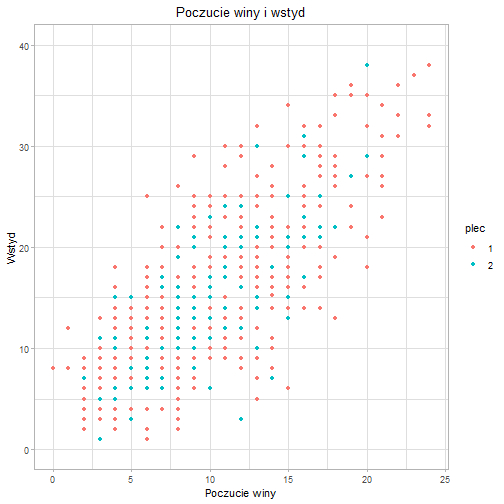
\includegraphics{Wawrowski_ADR_files/figure-latex/unnamed-chunk-20-1.pdf}

Najprostszym sposobem wizualizacji jest wykorzystanie funkcji \texttt{plot()}, niemniej taki wykres nie jest najpiękniejszy i trudno się go formatuje. Dużo lepiej skorzystać z pakietu \texttt{ggplot2}.

\begin{Shaded}
\begin{Highlighting}[]
\KeywordTok{ggplot}\NormalTok{(salary, }\KeywordTok{aes}\NormalTok{(}\DataTypeTok{x=}\NormalTok{YearsExperience, }\DataTypeTok{y=}\NormalTok{Salary)) }\OperatorTok{+}\StringTok{ }
\StringTok{  }\KeywordTok{geom_point}\NormalTok{() }\OperatorTok{+}
\StringTok{  }\KeywordTok{geom_smooth}\NormalTok{(}\DataTypeTok{method =} \StringTok{"lm"}\NormalTok{, }\DataTypeTok{se =} \OtherTok{FALSE}\NormalTok{) }\OperatorTok{+}
\StringTok{  }\KeywordTok{xlab}\NormalTok{(}\StringTok{"Doświadczenie"}\NormalTok{) }\OperatorTok{+}\StringTok{ }
\StringTok{  }\KeywordTok{ylab}\NormalTok{(}\StringTok{"Pensja"}\NormalTok{) }\OperatorTok{+}
\StringTok{  }\KeywordTok{xlim}\NormalTok{(}\DecValTok{0}\NormalTok{,}\DecValTok{12}\NormalTok{) }\OperatorTok{+}
\StringTok{  }\KeywordTok{ylim}\NormalTok{(}\DecValTok{35000}\NormalTok{, }\DecValTok{126000}\NormalTok{) }\OperatorTok{+}
\StringTok{  }\KeywordTok{theme_bw}\NormalTok{()}
\end{Highlighting}
\end{Shaded}

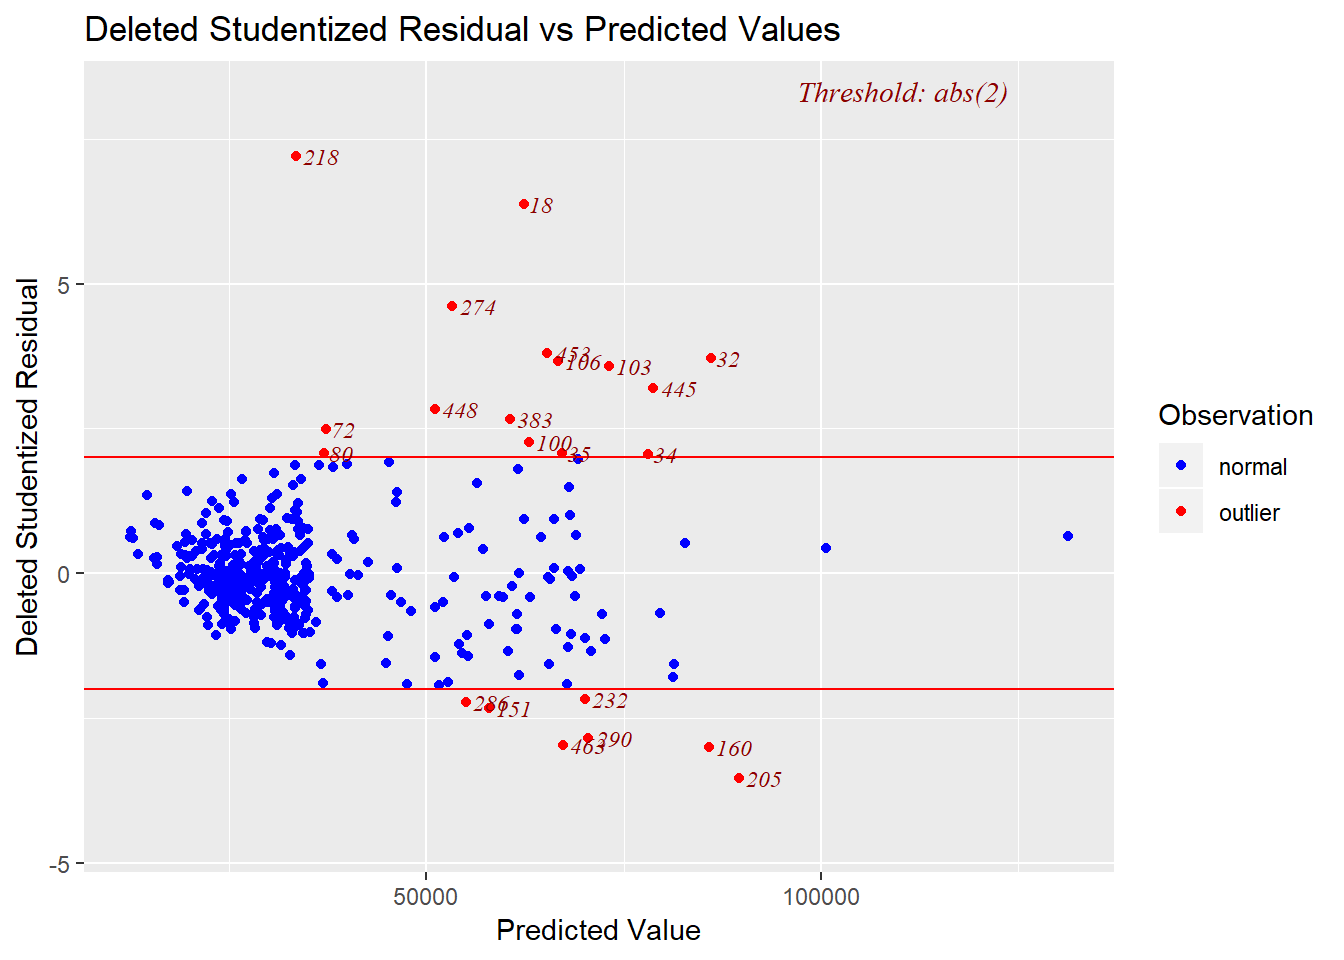
\includegraphics{Wawrowski_ADR_files/figure-latex/unnamed-chunk-21-1.pdf}

W argumentach funkcji \texttt{ggplot()} podajemy co wizualizujemy, natomiast sposób prezentacji ustalany jest przez funkcje \texttt{geom}. Funkcje \texttt{xlab()} i \texttt{ylab()} określają etykiety osi, a \texttt{xlim()} i \texttt{ylim()} wartości graniczne. Funkcje rozpoczynające się od \texttt{theme\_} określają wygląd wykresu.

Modelowanie rozpoczynamy od określenia zmiennej zależnej i niezależnej.

\begin{itemize}
\tightlist
\item
  zmienna zależna/objaśniana: pensja - \(y\)
\item
  zmienna niezależna/objaśniająca: doświadczenie - \(x\)
\end{itemize}

Szukamy teraz wzoru na prostą opisującą badane cechy.

Ogólna postać regresji prostej jest następująca:

\[\hat{y}_{i}=b_{1}x_{i}+b_{0}\]

gdzie \(\hat{y}\) oznacza wartość teoretyczną, leżącą na wyznaczonej prostej, \(x_i\) wartość zmiennej niezależnej, a \(b_1\) i \(b_0\) to współczynniki modelu.

Wobec tego wartości empiryczne \(y\) będą opisane formułą:

\[y_{i}=b_{1}x_{i}+b_{0}+u_{i}\]

w której \(u_i\) oznacza składnik resztowy wyliczany jako \(u_{i}=y_{i}-\hat{y}_{i}\).

\textbf{Współczynnik kierunkowy} \(b_1\) informuje o ile przeciętne zmieni się wartość zmiennej objaśnianej \(y\), gdy wartość zmiennej objaśniającej \(x\) wzrośnie o jednostkę.

\textbf{Wyraz wolny} \(b_0\) to wartość zmiennej objaśnianej \(y\), w sytuacji w której wartość zmiennej objaśniającej \(x\) będzie równa 0. Często interpretacja tego parametru nie ma sensu.

Następnie w R korzystamy z funkcji \texttt{lm}, w której należy określić zależność funkcyjną w formie: \texttt{zmienna\_zalezna\ \textasciitilde{}\ zmienna\ niezalezna}.

\begin{Shaded}
\begin{Highlighting}[]
\NormalTok{salary_model <-}\StringTok{ }\KeywordTok{lm}\NormalTok{(}\DataTypeTok{formula =}\NormalTok{ Salary }\OperatorTok{~}\StringTok{ }\NormalTok{YearsExperience, }\DataTypeTok{data =}\NormalTok{ salary)}
\KeywordTok{summary}\NormalTok{(salary_model)}
\end{Highlighting}
\end{Shaded}

\begin{verbatim}
## 
## Call:
## lm(formula = Salary ~ YearsExperience, data = salary)
## 
## Residuals:
##     Min      1Q  Median      3Q     Max 
## -7958.0 -4088.5  -459.9  3372.6 11448.0 
## 
## Coefficients:
##                 Estimate Std. Error t value Pr(>|t|)    
## (Intercept)      25792.2     2273.1   11.35 5.51e-12 ***
## YearsExperience   9450.0      378.8   24.95  < 2e-16 ***
## ---
## Signif. codes:  0 '***' 0.001 '**' 0.01 '*' 0.05 '.' 0.1 ' ' 1
## 
## Residual standard error: 5788 on 28 degrees of freedom
## Multiple R-squared:  0.957,  Adjusted R-squared:  0.9554 
## F-statistic: 622.5 on 1 and 28 DF,  p-value: < 2.2e-16
\end{verbatim}

Na podstawie otrzymanego wyniku dokonujemy interpretacji parametrów.

\begin{itemize}
\tightlist
\item
  b1 = 9450 - wzrost doświadczenia o rok powoduje przeciętny wzrost pensji o 9450 \$
\item
  b0 = 25792,2 - pracownik o doświadczeniu 0 lat uzyska pensję w wysokości 25792,2 \$
\end{itemize}

Trzy gwiazki przy współczynniku \(b_1\) oznaczają, że doświadczenie ma istotny wpływ na wartości pensji. Wyraz wolny także jest istotny, natomiast ogólnie nie jest wymagana jesgo istotność.

Oprócz interpretacji współczynników ważne są jeszcze inne miary jakości modelu.

\textbf{Odchylenie standardowe składnika resztowego} jest pierwiastkiem z sumy kwadratów reszt podzielonej przez liczbę obserwacji pomniejszoną o 2:

\[S_{u}=\sqrt{\frac{\sum\limits_{i=1}^{n}{(y_{i}-\hat{y}_{i})^2}}{n-2}}\]

Błąd resztowy (odchylenie standardowe składnika resztowego) \(S_u\) wynosi 5788\$, co oznacza, że wartości obliczone na podstawie modelu różnią się od rzeczywistości średnio o +/- 5788
\$

\textbf{Współczynnik determinacji} określa, jaki procent wariancji zmiennej objaśnianej został wyjaśniony przez funkcję regresji. \(R^2\) przyjmuje wartości z przedziału \(<0;1>\) ( \(<0\%;100\%>\) ), przy czym model regresji tym lepiej opisuje zachowanie się badanej zmiennej objaśnianej, im \(R^2\) jest bliższy jedności (bliższy 100\%)

\[R^2=1-\frac{\sum\limits_{i=1}^{n}{(y_{i}-\hat{y}_{i})^2}}{\sum\limits_{i=1}^{n}{(y_{i}-\bar{y}_{i})^2}}\]

Współczynnik \(R^2\) (multiple R-squared) wynosi 0,957 czyli doświadczenie wyjaśnia 95,7\% zmienności pensji

Na podstawie tego modelu dokonamy wyznaczenia wartości teoretycznych dla kilku wybranych wartości doświadczenia. Nowe wartości muszą być w postaci zbioru danych, zatem tworzymy nową ramkę danych.

\begin{Shaded}
\begin{Highlighting}[]
\NormalTok{nowiPracownicy <-}\StringTok{ }\KeywordTok{data.frame}\NormalTok{(}\DataTypeTok{YearsExperience=}\KeywordTok{c}\NormalTok{(}\DecValTok{8}\NormalTok{,}\DecValTok{10}\NormalTok{,}\DecValTok{11}\NormalTok{))}

\KeywordTok{predict}\NormalTok{(salary_model, nowiPracownicy)}
\end{Highlighting}
\end{Shaded}

\begin{verbatim}
##        1        2        3 
## 101391.9 120291.8 129741.8
\end{verbatim}

Tym sposobem uzyskujemy następujące widełki:

\begin{itemize}
\tightlist
\item
  pracownik o 8 latach doświadczenia - proponowana pensja 101391,9 \$ +/- 5788
  \$
\item
  pracownik o 10 latach doświadczenia - proponowana pensja 120291,8 \$ +/- 5788
  \$
\item
  pracownik o 11 latach doświadczenia - proponowana pensja 129741,8 \$ +/- 5788
  \$
\end{itemize}

W powyższym przykładzie prognozowane wartości pojawiły się w konsoli, natomiast w sytuacji, w której chcielibyśmy wykonać predykcję dla bardzo wielu nowych wartości to warto te prognozowane wartości umieścić od razu w zbiorze danych. Można to zrobić w następujący sposób:

\begin{Shaded}
\begin{Highlighting}[]
\NormalTok{nowiPracownicy <-}\StringTok{ }\NormalTok{nowiPracownicy }\OperatorTok\StringTok{ }
\StringTok{  }\KeywordTok{mutate}\NormalTok{(}\DataTypeTok{salary_pred=}\KeywordTok{predict}\NormalTok{(}\DataTypeTok{object =}\NormalTok{ salary_model, }\DataTypeTok{newdata =}\NormalTok{ .))}

\NormalTok{nowiPracownicy}
\end{Highlighting}
\end{Shaded}

\begin{verbatim}
##   YearsExperience salary_pred
## 1               8    101391.9
## 2              10    120291.8
## 3              11    129741.8
\end{verbatim}

W powyższym kodzie symbol \texttt{.} oznacza analizowany zbiór danych, zatem nie ma potrzeby powtarzania jego nazwy.

\hypertarget{zadanie}{%
\subsection{Zadanie}\label{zadanie}}

Dla danych dotyczących \href{data/sklep77.xlsx}{sklepu nr 77} opracuj model zależności sprzedaży od liczby klientów. Ile wynosi teoretyczna sprzedaż w dniach, w których liczba klientów będzie wynosiła 560, 740, 811 oraz 999 osób?

\hypertarget{regresja-wieloraka}{%
\section{Regresja wieloraka}\label{regresja-wieloraka}}

Ogólna postać regresji wielorakiej jest następująca:

\[\hat{y}_{i}=b_{1}x_{1i}+b_{2}x_{2i}+...+b_{k}x_{ki}+b_{0}\]

W tym przypadku nie wyznaczamy prostej tylko \(k\)-wymiarową przestrzeń.

Na podstawie danych dotyczących \href{data/pracownicy.xlsx}{zatrudnienia} opracuj model, w którym zmienną zależną jest bieżące wynagrodzenie. Za pomocą regresji określimy jakie cechy mają istotny wpływ na to wynagrodzenie.

Opis zbioru:

\begin{itemize}
\tightlist
\item
  id - kod pracownika
\item
  plec - płeć pracownika (0 - mężczyzna, 1 - kobieta)
\item
  data\_urodz - data urodzenia
\item
  edukacja - wykształcenie (w latach nauki)
\item
  kat\_pracownika - grupa pracownicza (1 - specjalista, 2 - menedżer, 3 - konsultant)
\item
  bwynagrodzenie - bieżące wynagrodzenie
\item
  pwynagrodzenie - początkowe wynagrodzenie
\item
  staz - staż pracy (w miesiącach)
\item
  doswiadczenie - poprzednie zatrudnienie (w miesiącach)
\item
  zwiazki - przynależność do związków zawodowych (0 - nie, 1 - tak)
\item
  wiek - wiek (w latach)
\end{itemize}

Rozpoczynamy od wczytania danych,

\begin{Shaded}
\begin{Highlighting}[]
\NormalTok{pracownicy <-}\StringTok{ }\KeywordTok{read_xlsx}\NormalTok{(}\StringTok{"data/pracownicy.xlsx"}\NormalTok{)}

\NormalTok{pracownicy2 <-}\StringTok{ }\NormalTok{pracownicy }\OperatorTok
\StringTok{  }\KeywordTok{filter}\NormalTok{(}\OperatorTok{!}\KeywordTok{is.na}\NormalTok{(wiek)) }\OperatorTok
\StringTok{  }\KeywordTok{select}\NormalTok{(}\OperatorTok{-}\NormalTok{id, }\OperatorTok{-}\NormalTok{data_urodz) }\OperatorTok
\StringTok{  }\KeywordTok{mutate}\NormalTok{(}\DataTypeTok{plec=}\KeywordTok{as.factor}\NormalTok{(plec),}
         \DataTypeTok{kat_pracownika=}\KeywordTok{as.factor}\NormalTok{(kat_pracownika),}
         \DataTypeTok{zwiazki=}\KeywordTok{as.factor}\NormalTok{(zwiazki))}

\KeywordTok{summary}\NormalTok{(pracownicy2)}
\end{Highlighting}
\end{Shaded}

\begin{verbatim}
##  plec       edukacja     kat_pracownika bwynagrodzenie   pwynagrodzenie 
##  0:257   Min.   : 8.00   1:362          Min.   : 15750   Min.   : 9000  
##  1:216   1st Qu.:12.00   2: 27          1st Qu.: 24000   1st Qu.:12450  
##          Median :12.00   3: 84          Median : 28800   Median :15000  
##          Mean   :13.49                  Mean   : 34418   Mean   :17009  
##          3rd Qu.:15.00                  3rd Qu.: 37050   3rd Qu.:17490  
##          Max.   :21.00                  Max.   :135000   Max.   :79980  
##       staz       doswiadczenie    zwiazki      wiek      
##  Min.   :63.00   Min.   :  0.00   0:369   Min.   :24.00  
##  1st Qu.:72.00   1st Qu.: 19.00   1:104   1st Qu.:30.00  
##  Median :81.00   Median : 55.00           Median :33.00  
##  Mean   :81.14   Mean   : 95.95           Mean   :38.67  
##  3rd Qu.:90.00   3rd Qu.:139.00           3rd Qu.:47.00  
##  Max.   :98.00   Max.   :476.00           Max.   :66.00
\end{verbatim}

W zmiennej wiek występował brak danych, który został usunięty. Usunięto także kolumny, które nie przydadzą się w modelowaniu. Ponadto dokonujemy przekształcenia typu cech, które są jakościowe (płeć, kat\_pracownika, zwiazki) z typu liczbowego na czynnik/faktor. Taka modyfikacja powoduje, że ta cecha będzie przez model traktowana jako zmienna dychotomiczna (zerojedynkowa). Proces trasformacji takiej cechy jest pokazany poniżej.

Oryginalny zbiór

\begin{longtable}[]{@{}ll@{}}
\toprule
id & stanowisko\tabularnewline
\midrule
\endhead
1 & specjalista\tabularnewline
2 & menedżer\tabularnewline
3 & specjalista\tabularnewline
4 & konsultant\tabularnewline
5 & konsultant\tabularnewline
\bottomrule
\end{longtable}

Zmienna zerojedynkowa

\begin{longtable}[]{@{}lll@{}}
\toprule
id & menedżer & konsultant\tabularnewline
\midrule
\endhead
1 & 0 & 0\tabularnewline
2 & 1 & 0\tabularnewline
3 & 0 & 0\tabularnewline
4 & 0 & 1\tabularnewline
5 & 0 & 1\tabularnewline
\bottomrule
\end{longtable}

W modelu zmienna zależna to \texttt{bwynagrodzenie}, natomiast jako zmienne niezależne bierzemy pod uwagę wszystkie pozostałe cechy. W celu uniknięcia notacji naukowej w uzyskiwanych wynikach dodajemy opcję \texttt{options(scipen\ =\ 5)}.

\begin{Shaded}
\begin{Highlighting}[]
\KeywordTok{options}\NormalTok{(}\DataTypeTok{scipen =} \DecValTok{5}\NormalTok{)}

\NormalTok{model <-}\StringTok{ }\KeywordTok{lm}\NormalTok{(bwynagrodzenie }\OperatorTok{~}\StringTok{ }\NormalTok{., pracownicy2)}
\KeywordTok{summary}\NormalTok{(model)}
\end{Highlighting}
\end{Shaded}

\begin{verbatim}
## 
## Call:
## lm(formula = bwynagrodzenie ~ ., data = pracownicy2)
## 
## Residuals:
##    Min     1Q Median     3Q    Max 
## -23185  -3041   -705   2591  46295 
## 
## Coefficients:
##                    Estimate  Std. Error t value Pr(>|t|)    
## (Intercept)     -4764.87418  3590.49652  -1.327  0.18514    
## plec1           -1702.43743   796.51779  -2.137  0.03309 *  
## edukacja          482.43603   160.83977   2.999  0.00285 ** 
## kat_pracownika2  6643.17910  1638.06138   4.056 5.87e-05 ***
## kat_pracownika3 11169.64519  1372.73990   8.137 3.77e-15 ***
## pwynagrodzenie      1.34021     0.07317  18.315  < 2e-16 ***
## staz              154.50876    31.65933   4.880 1.46e-06 ***
## doswiadczenie     -15.77375     5.78369  -2.727  0.00663 ** 
## zwiazki1        -1011.55276   787.80884  -1.284  0.19978    
## wiek              -64.78787    47.88015  -1.353  0.17668    
## ---
## Signif. codes:  0 '***' 0.001 '**' 0.01 '*' 0.05 '.' 0.1 ' ' 1
## 
## Residual standard error: 6809 on 463 degrees of freedom
## Multiple R-squared:  0.8444, Adjusted R-squared:  0.8414 
## F-statistic: 279.1 on 9 and 463 DF,  p-value: < 2.2e-16
\end{verbatim}

Tak zbudowany model wyjaśnia 84,4\% zmienności bieżącego wynagrodzenia, ale nie wszystkie zmienne są w tym modelu istotne.

Parametry regresji mają następujące interpretacje:

\begin{itemize}
\tightlist
\item
  plec1 - kobiety zarabiają przeciętnie o 1702,44 zł mniej niż mężczyźni,
\item
  edukacja - wzrost liczby lat nauki o rok powoduje średni wzrost bieżącego wynagrodzenia o 482,44 zł
\item
  kat\_pracownika2 - pracownicy o kodzie 2 (menedżer) zarabiają średnio o 6643,18 zł więcej niż pracownik o kodzie 1 (specjalista)
\item
  kat\_pracownika2 - pracownicy o kodzie 3 (konsultant) zarabiają średnio o 11169,65 zł więcej niż pracownik o kodzie 1 (specjalista)
\item
  pwynagrodzenie - wzrost początkowego wynagrodzenia o 1 zł powoduje przeciętny wzrost bieżącego wynagrodzenia o 1,34 zł
\item
  staz - wzrost stażu pracy o miesiąc skutkuje przeciętnym wzrostem bieżącego wynagrodzenia o 154,51 zł
\item
  doswiadcznie - wzrost doświadczenia o miesiąc powoduje średni spadek bieżącego wynagrodzenia o 15,77 zł
\item
  zwiazki1 - pracownicy należący do związków zawodowych zarabiają średnio o 1011,55 zł mniej aniżeli pracownicy, którzy do związków nie zależą
\item
  wiek - wzrost wieku pracownika o 1 rok to przeciętnym spadek bieżącego wynagrodzenia o 64,79 zł
\end{itemize}

Wszystkie te interpretacje obowiązują przy założeniu \emph{ceteris paribus} - przy pozostałych warunkach niezmienionych.

Ten model wymaga oczywiście ulepszenia do czego wykorzystamy pakiet \href{https://cran.r-project.org/web/packages/olsrr/index.html}{olsrr}.

Pierwszą kwestią, którą się zajmiemy jest współliniowość zmiennych. W regresji zmienne objaśniające powinny być jak najbardziej skorelowane ze zmienną objaśnianą, a możliwie nieskorelowane ze sobą. W związku z tym wybieramy ze zbioru wyłącznie cechy ilościowe, dla którym wyznaczymy współczynnik korelacji liniowej Pearsona. Do wizualizacji tych wartości wykorzystamy pakiet \href{https://cran.r-project.org/web/packages/corrplot/}{corrplot} służący do wizualizacji współczynnika korelacji.

\begin{Shaded}
\begin{Highlighting}[]
\KeywordTok{library}\NormalTok{(corrplot)}
\KeywordTok{library}\NormalTok{(olsrr)}

\NormalTok{korelacje <-}\StringTok{ }\NormalTok{pracownicy2 }\OperatorTok
\StringTok{  }\KeywordTok{select}\NormalTok{(}\OperatorTok{-}\KeywordTok{c}\NormalTok{(plec, kat_pracownika, zwiazki)) }\OperatorTok
\StringTok{  }\KeywordTok{cor}\NormalTok{()}

\KeywordTok{corrplot}\NormalTok{(korelacje, }\DataTypeTok{method =} \StringTok{"number"}\NormalTok{, }\DataTypeTok{type =} \StringTok{"upper"}\NormalTok{)}
\end{Highlighting}
\end{Shaded}

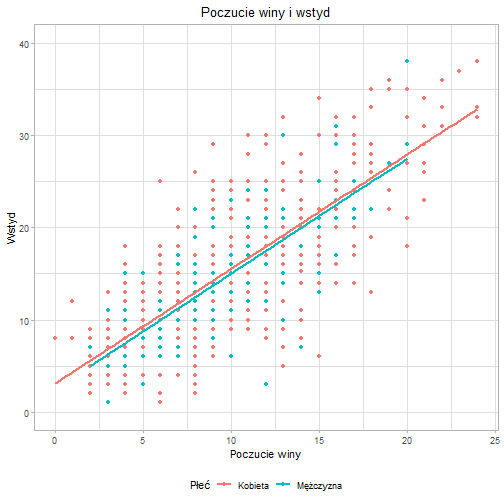
\includegraphics{Wawrowski_ADR_files/figure-latex/unnamed-chunk-27-1.pdf}

Możemy zauważyć, że wartości bieżącego wynagrodzenia są najsilniej skorelowane w wartościami wynagrodzenia początkowego. Także doświadczenie i wiek są silnie ze sobą związane, co może sugerować, że obie zmienne wnoszą do modelu podobną informację.

W związku z tym powinniśmy wyeliminować niektóre zmienne z modelu pozostawiając te najważniejsze. Wyróżnia się trzy podejścia do tego zagadnienia:

\begin{itemize}
\tightlist
\item
  ekspercki dobór cech,
\item
  budowa wszystkich możliwych modeli i wybór najlepszego według określonego kryterium,
\item
  regresja krokowa.
\end{itemize}

W przypadku budowy wszystkich możliwych modeli należy pamiętać o rosnącej wykładniczo liczbie modeli: \(2^p-1\), gdzie \(p\) oznacza liczbę zmiennych objaśniających. w rozważanym przypadku liczba modeli wynosi 255.

\begin{Shaded}
\begin{Highlighting}[]
\NormalTok{wszystkie_modele <-}\StringTok{ }\KeywordTok{ols_step_all_possible}\NormalTok{(model)}
\end{Highlighting}
\end{Shaded}

W uzyskanym zbiorze danych są informacje o numerze modelu, liczbie użytych zmiennych, nazwie tych zmiennych oraz wiele miar jakości. Te, które warto wziąć pod uwagę to przede wszystkim:

\begin{itemize}
\tightlist
\item
  \texttt{rsquare} - współczynnik R-kwadrat,
\item
  \texttt{aic} - kryterium informacyjne Akaike,
\item
  \texttt{msep} - błąd średniokwadratowy predykcji.
\end{itemize}

Najwyższa wartość współczynnika \(R^2\) związana jest z modelem zawierającym wszystkie dostępne zmienne objaśniające. Jest to pewna niedoskonałość tej miary, która rośnie wraz z liczbą zmiennych w modelu, nawet jeśli te zmienne nie są istotne.

W przypadku kryteriów informacyjnych oraz błędu średniokwadratowego interesują nas jak najmniejsze wartości. Wówczas jako najlepszy należy wskazać model nr 219 zawierający 6 zmiennych objaśniających.

Metodą, która także pozwoli uzyskać optymalny model, ale przy mniejszym obciążeniu obliczeniowym jest regresja krokowa polegająca na krokowym budowaniu modelu.

\begin{Shaded}
\begin{Highlighting}[]
\KeywordTok{ols_step_both_aic}\NormalTok{(model)}
\end{Highlighting}
\end{Shaded}

\begin{verbatim}
## Stepwise Selection Method 
## -------------------------
## 
## Candidate Terms: 
## 
## 1 . plec 
## 2 . edukacja 
## 3 . kat_pracownika 
## 4 . pwynagrodzenie 
## 5 . staz 
## 6 . doswiadczenie 
## 7 . zwiazki 
## 8 . wiek 
## 
## 
## Variables Entered/Removed: 
## 
## - pwynagrodzenie added 
## - kat_pracownika added 
## - doswiadczenie added 
## - staz added 
## - edukacja added 
## - plec added 
## 
## No more variables to be added or removed.
\end{verbatim}

\begin{verbatim}
## 
## 
##                                            Stepwise Summary                                            
## -----------------------------------------------------------------------------------------------------
## Variable           Method       AIC             RSS               Sum Sq          R-Sq      Adj. R-Sq 
## -----------------------------------------------------------------------------------------------------
## pwynagrodzenie    addition    9862.260    31053506813.535    106862706669.340    0.77484      0.77436 
## kat_pracownika    addition    9786.152    26215474648.689    111700738834.186    0.80992      0.80870 
## doswiadczenie     addition    9743.487    23853248017.651    114062965465.224    0.82705      0.82557 
## staz              addition    9719.469    22576592070.620    115339621412.255    0.83630      0.83455 
## edukacja          addition    9707.338    21912088629.084    116004124853.791    0.84112      0.83907 
## plec              addition    9703.188    21629051655.016    116287161827.859    0.84317      0.84081 
## -----------------------------------------------------------------------------------------------------
\end{verbatim}

Otrzymany w ten sposób model jest tożsamy z modelem charakteryzującym się najlepszymi miarami jakości spośród zbioru wszystkich możliwych modeli:

\begin{Shaded}
\begin{Highlighting}[]
\NormalTok{wybrany_model <-}\StringTok{ }\KeywordTok{lm}\NormalTok{(bwynagrodzenie }\OperatorTok{~}\StringTok{ }\NormalTok{pwynagrodzenie }\OperatorTok{+}\StringTok{ }\NormalTok{kat_pracownika }\OperatorTok{+}\StringTok{ }\NormalTok{doswiadczenie }\OperatorTok{+}\StringTok{ }\NormalTok{staz }\OperatorTok{+}\StringTok{ }\NormalTok{plec }\OperatorTok{+}\StringTok{ }\NormalTok{edukacja, }\DataTypeTok{data =}\NormalTok{ pracownicy2)}
\KeywordTok{summary}\NormalTok{(wybrany_model)}
\end{Highlighting}
\end{Shaded}

\begin{verbatim}
## 
## Call:
## lm(formula = bwynagrodzenie ~ pwynagrodzenie + kat_pracownika + 
##     doswiadczenie + staz + plec + edukacja, data = pracownicy2)
## 
## Residuals:
##    Min     1Q Median     3Q    Max 
## -22922  -3300   -673   2537  46524 
## 
## Coefficients:
##                  Estimate Std. Error t value Pr(>|t|)    
## (Intercept)     -6547.147   3402.860  -1.924  0.05496 .  
## pwynagrodzenie      1.342      0.073  18.382  < 2e-16 ***
## kat_pracownika2  6734.992   1631.122   4.129 4.32e-05 ***
## kat_pracownika3 11226.635   1368.413   8.204 2.30e-15 ***
## doswiadczenie     -22.302      3.571  -6.246 9.51e-10 ***
## staz              147.865     31.461   4.700 3.43e-06 ***
## plec1           -1878.949    761.703  -2.467  0.01399 *  
## edukacja          501.391    160.270   3.128  0.00187 ** 
## ---
## Signif. codes:  0 '***' 0.001 '**' 0.01 '*' 0.05 '.' 0.1 ' ' 1
## 
## Residual standard error: 6820 on 465 degrees of freedom
## Multiple R-squared:  0.8432, Adjusted R-squared:  0.8408 
## F-statistic: 357.1 on 7 and 465 DF,  p-value: < 2.2e-16
\end{verbatim}

Uzyskany model charakteryzuje się nieznacznie większym błędem resztowym od modelu ze wszystkimi zmiennymi, ale wszystkie zmienne są istotne. Wyraz wolny \texttt{(Intercept)} nie musi być istotny w modelu.

Wróćmy jeszcze na chwilę do tematu współliniowości zmiennych objaśniających:

\begin{Shaded}
\begin{Highlighting}[]
\KeywordTok{ols_vif_tol}\NormalTok{(wybrany_model)}
\end{Highlighting}
\end{Shaded}

\begin{verbatim}
## # A tibble: 7 x 3
##   Variables       Tolerance   VIF
##   <chr>               <dbl> <dbl>
## 1 pwynagrodzenie      0.298  3.36
## 2 kat_pracownika2     0.687  1.46
## 3 kat_pracownika3     0.360  2.78
## 4 doswiadczenie       0.705  1.42
## 5 staz                0.986  1.01
## 6 plec1               0.683  1.46
## 7 edukacja            0.461  2.17
\end{verbatim}

Współczynnik tolerancji wskazuje na procent niewyjaśnionej zmienności danej zmiennej przez pozostałe zmienne objaśniające. Przykładowo współczynnik tolerancji dla początkowego wynagrodzenia wynosi 0,2980, co oznacza, że 30\% zmienności początkowego wynagrodzenia nie jest wyjaśnione przez pozostałe zmienne w modelu. Z kolei współczynnik VIF jest obliczany na podstawie wartości współczynnika tolerancji i wskazuje o ile wariancja szacowanego współczynnika regresji jest podwyższona z powodu współliniowości danej zmiennej objaśniającej z pozostałymi zmiennymi objaśniającymi. Wartość współczynnika VIF powyżej 4 należy uznać za wskazującą na współliniowość. W analizowanym przypadku takie zmienne nie występują.

Ocena siły wpływu poszczególnych zmiennych objaśniających na zmienną objaśnianą w oryginalnej postaci modelu nie jest możliwa. Należy wyznaczyć standaryzowane współczynniki beta, które wyliczane są na danych standaryzowanych, czyli takich, które są pozbawione jednostek i cechują się średnią równą 0, a odchyleniem standardowym równym 1. Standaryzacja ma sens tylko dla cech numerycznych, w związku z czym korzystamy z funkcji \texttt{mutate\_if()}, która jako pierwszy argument przyjmuje warunek, który ma być spełniony, aby była zastosowane przekształcenie podawane jako drugi argument.

\begin{Shaded}
\begin{Highlighting}[]
\NormalTok{pracownicy2_std <-}\StringTok{ }\NormalTok{pracownicy2 }\OperatorTok
\StringTok{  }\KeywordTok{mutate_if}\NormalTok{(is.numeric, scale)}

\NormalTok{wybrany_model_std <-}\StringTok{ }\KeywordTok{lm}\NormalTok{(bwynagrodzenie }\OperatorTok{~}\StringTok{ }\NormalTok{pwynagrodzenie }\OperatorTok{+}\StringTok{ }\NormalTok{kat_pracownika }\OperatorTok{+}\StringTok{ }
\StringTok{                          }\NormalTok{doswiadczenie }\OperatorTok{+}\StringTok{ }\NormalTok{staz }\OperatorTok{+}\StringTok{ }\NormalTok{plec }\OperatorTok{+}\StringTok{ }\NormalTok{edukacja, }\DataTypeTok{data =}\NormalTok{ pracownicy2_std)}
\KeywordTok{summary}\NormalTok{(wybrany_model_std)}
\end{Highlighting}
\end{Shaded}

\begin{verbatim}
## 
## Call:
## lm(formula = bwynagrodzenie ~ pwynagrodzenie + kat_pracownika + 
##     doswiadczenie + staz + plec + edukacja, data = pracownicy2_std)
## 
## Residuals:
##      Min       1Q   Median       3Q      Max 
## -1.34098 -0.19306 -0.03939  0.14841  2.72171 
## 
## Coefficients:
##                 Estimate Std. Error t value Pr(>|t|)    
## (Intercept)     -0.08893    0.03144  -2.828  0.00488 ** 
## pwynagrodzenie   0.61842    0.03364  18.382  < 2e-16 ***
## kat_pracownika2  0.39400    0.09542   4.129 4.32e-05 ***
## kat_pracownika3  0.65677    0.08005   8.204 2.30e-15 ***
## doswiadczenie   -0.13657    0.02187  -6.246 9.51e-10 ***
## staz             0.08691    0.01849   4.700 3.43e-06 ***
## plec1           -0.10992    0.04456  -2.467  0.01399 *  
## edukacja         0.08464    0.02706   3.128  0.00187 ** 
## ---
## Signif. codes:  0 '***' 0.001 '**' 0.01 '*' 0.05 '.' 0.1 ' ' 1
## 
## Residual standard error: 0.399 on 465 degrees of freedom
## Multiple R-squared:  0.8432, Adjusted R-squared:  0.8408 
## F-statistic: 357.1 on 7 and 465 DF,  p-value: < 2.2e-16
\end{verbatim}

Spośród cech ilościowych największy wpływ na zmienną objaśnianą mają wartości wynagrodzenia początkowego, staż, edukacja i na końcu doświadczenie.

Reszty czyli różnice pomiędzy obserwowanymi wartościami zmiennej objaśnianej, a wartościami wynikającymi z modelu w klasycznej metodzie najmniejszych kwadratów powinny być zbliżone do rozkładu normalnego. Oznacza to, że najwięcej reszt powinno skupiać się wokół zerowych różnic, natomiast jak najmniej powinno być wartości modelowych znacznie różniących się od tych rzeczywistych.

\begin{Shaded}
\begin{Highlighting}[]
\KeywordTok{ols_plot_resid_hist}\NormalTok{(wybrany_model)}
\end{Highlighting}
\end{Shaded}

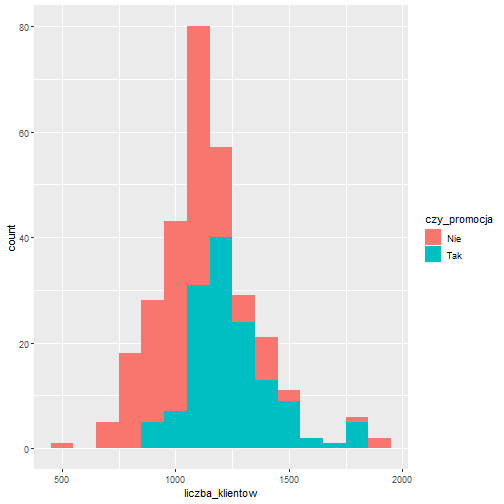
\includegraphics{Wawrowski_ADR_files/figure-latex/unnamed-chunk-33-1.pdf}

Reszty w naszym modelu wydają się być zbliżone do rozkładu normalnego. Jednoznaczną odpowiedź da jednak odpowiedni test.

\begin{Shaded}
\begin{Highlighting}[]
\KeywordTok{ols_test_normality}\NormalTok{(wybrany_model)}
\end{Highlighting}
\end{Shaded}

\begin{verbatim}
## -----------------------------------------------
##        Test             Statistic       pvalue  
## -----------------------------------------------
## Shapiro-Wilk              0.868          0.0000 
## Kolmogorov-Smirnov        0.1092         0.0000 
## Cramer-von Mises         42.5504         0.0001 
## Anderson-Darling         13.0233         0.0000 
## -----------------------------------------------
\end{verbatim}

Hipoteza zerowa w tych testach mówi o zgodności rozkładu reszt z rozkładem normalnym. Na podstawie wartości p, które są mniejsze od \(\alpha=0,05\) stwierdzamy, że są podstawy do odrzucenia tej hipotezy czyli reszty z naszego modelu nie mają rozkładu normalnego. W diagnostyce przyczyn takiego stanu rzeczy pomoże nam wykres kwantyl-kwantyl:

\begin{Shaded}
\begin{Highlighting}[]
\KeywordTok{ols_plot_resid_qq}\NormalTok{(wybrany_model)}
\end{Highlighting}
\end{Shaded}

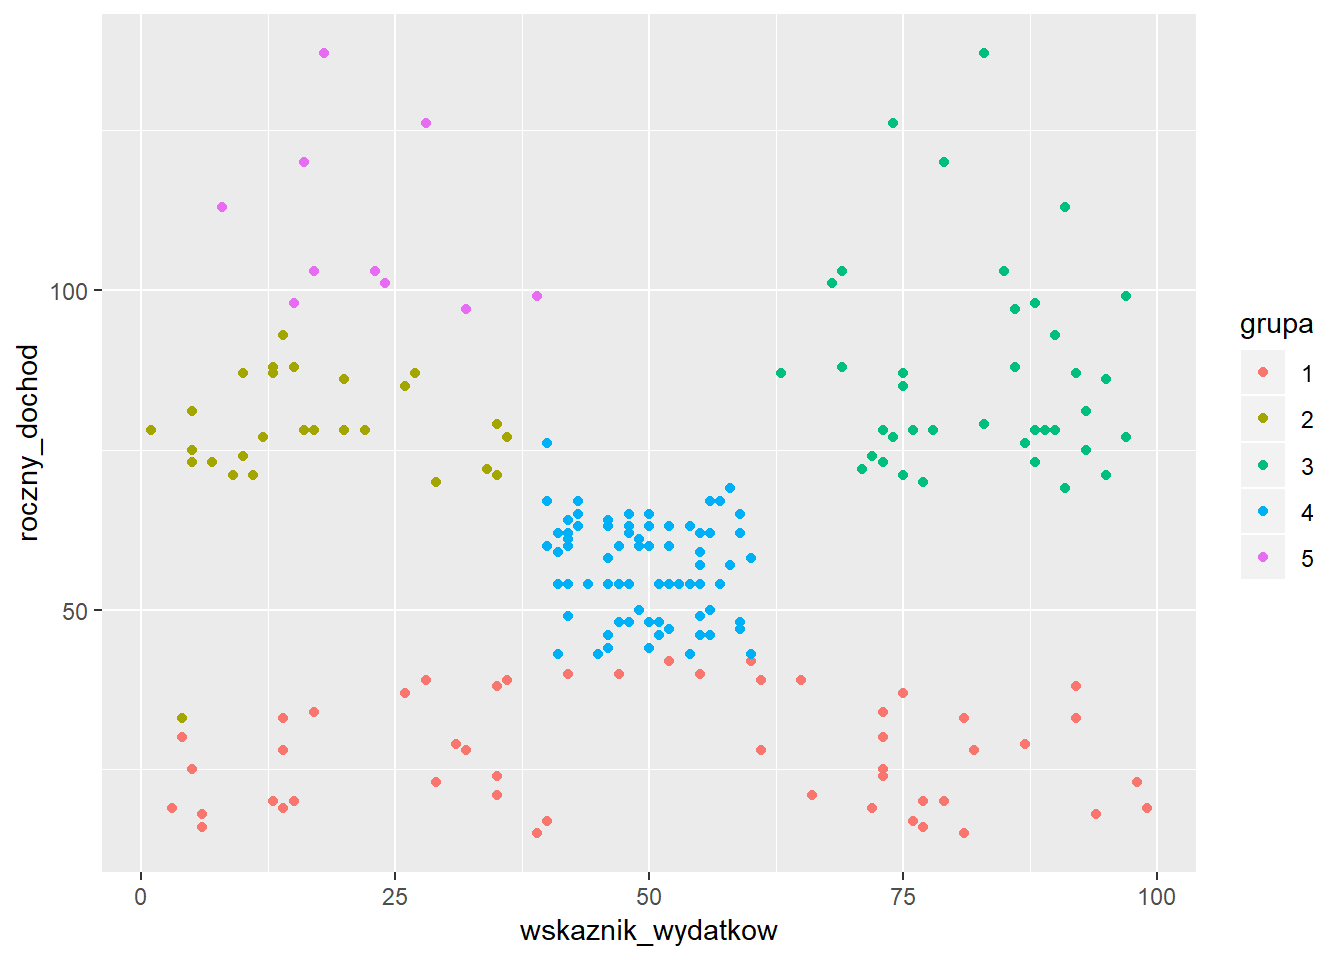
\includegraphics{Wawrowski_ADR_files/figure-latex/unnamed-chunk-35-1.pdf}

Gdyby wszystkie punkty leżały na prostej to oznaczałoby to normalność rozkładu reszt. Tymczasem po lewej i prawej stronie tego wykresu znajdują się potencjalne wartości odstające, które znacznie wpływają na rozkład reszt modelu.

Wartości odstające można ustalić na podstawie wielu kryteriów. Do jednych z najbardziej popularnych należy odległość Cooka:

\begin{Shaded}
\begin{Highlighting}[]
\NormalTok{cook <-}\StringTok{ }\KeywordTok{ols_plot_cooksd_bar}\NormalTok{(wybrany_model)}
\end{Highlighting}
\end{Shaded}

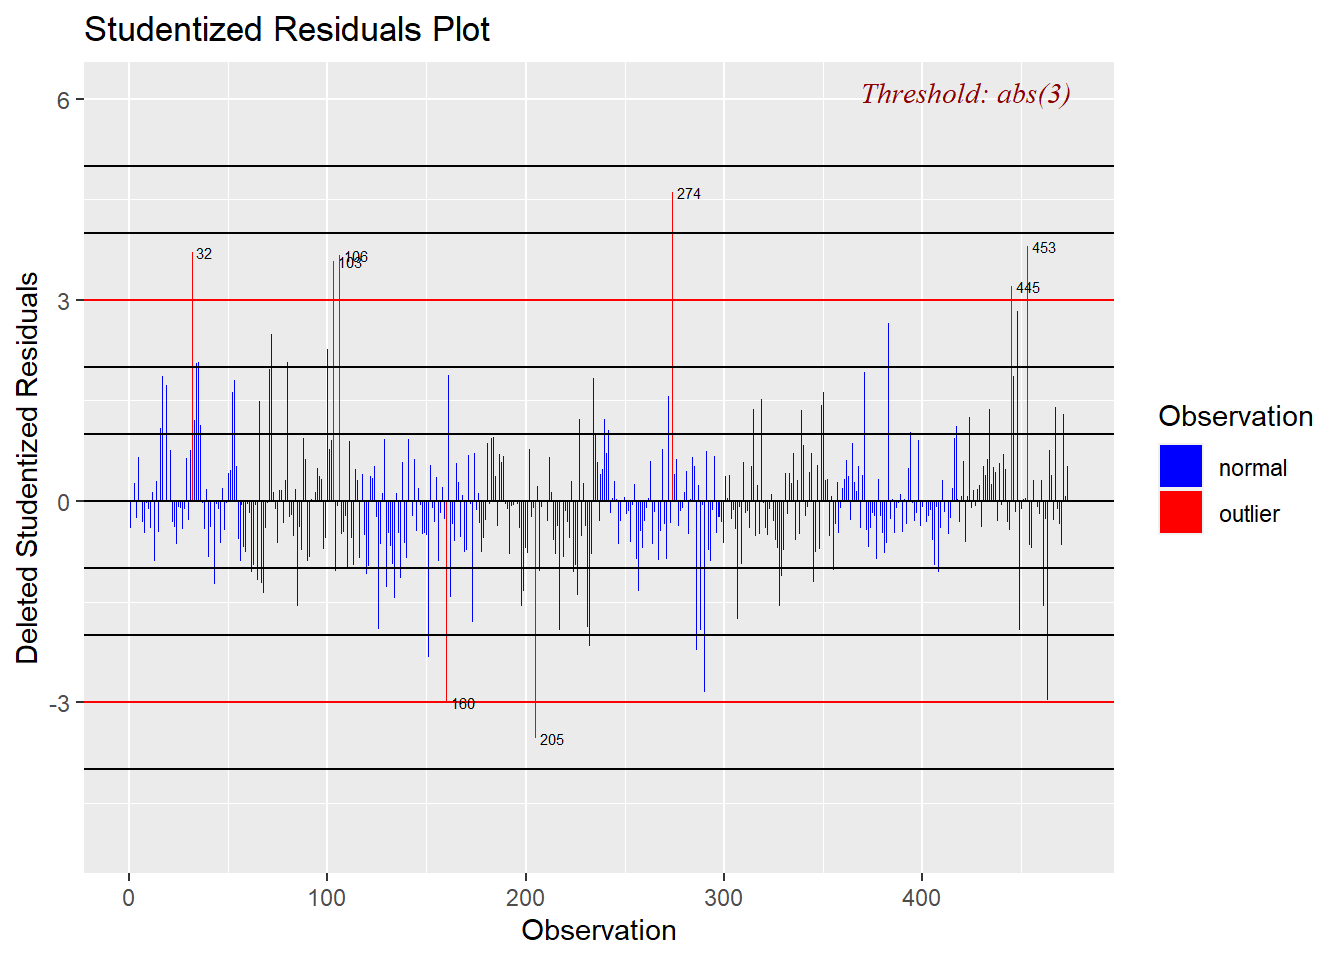
\includegraphics{Wawrowski_ADR_files/figure-latex/unnamed-chunk-36-1.pdf}

Przypisanie tej funkcji do obiektu zwraca nam tabelę z numerami zidentyfikowanych obserwacji wpływowych. W przypadku odległości Cooka jest to 35 obserwacji.

Inną miarą są reszty studentyzowane.

\begin{Shaded}
\begin{Highlighting}[]
\NormalTok{stud3 <-}\StringTok{ }\KeywordTok{ols_plot_resid_stud}\NormalTok{(wybrany_model)}
\end{Highlighting}
\end{Shaded}

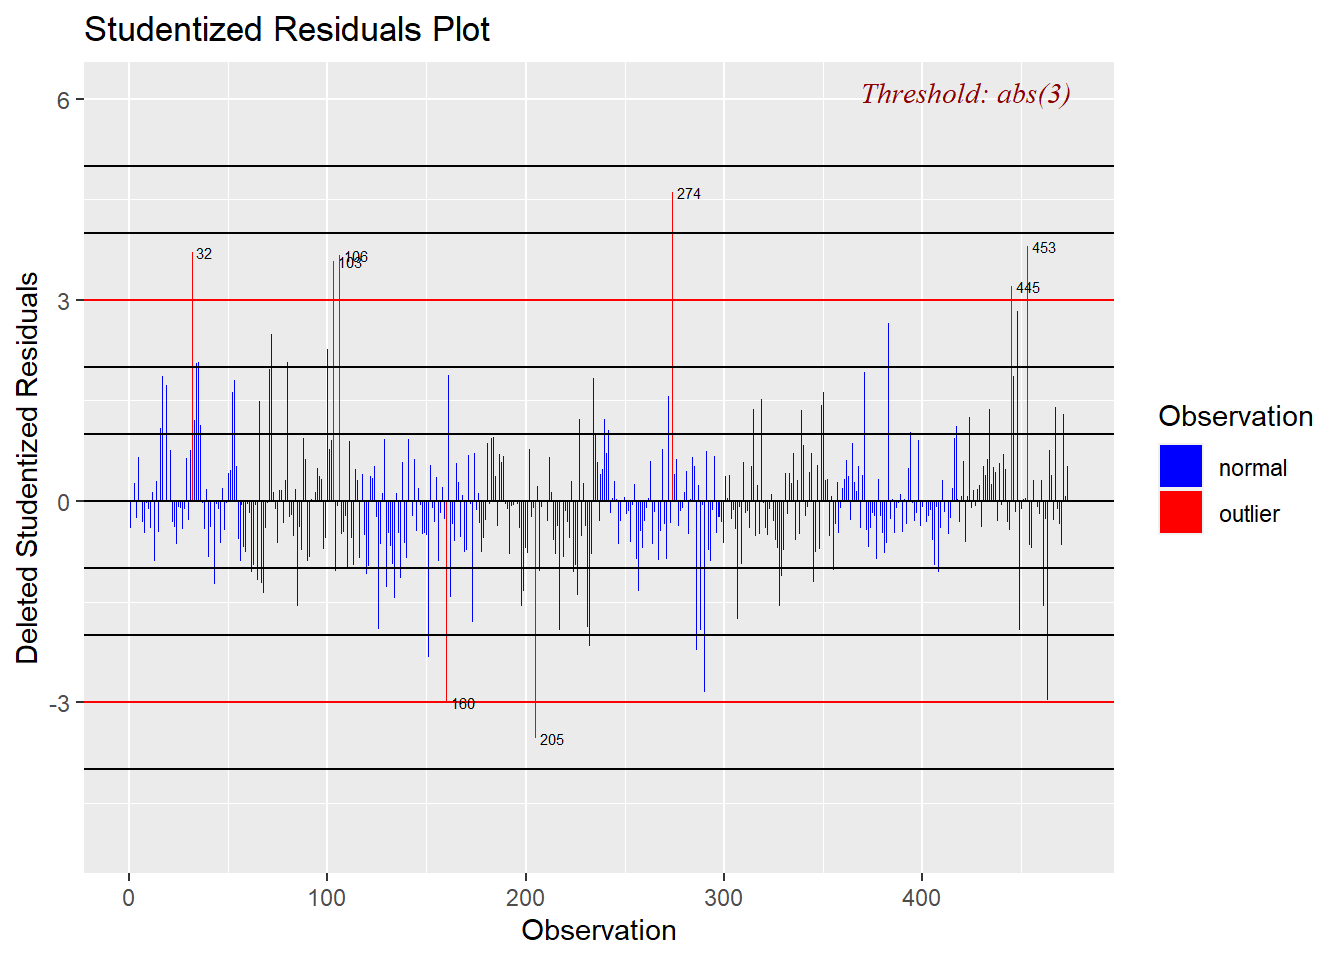
\includegraphics{Wawrowski_ADR_files/figure-latex/unnamed-chunk-37-1.pdf}

Wyżej wykorzystana funkcja jako kryterium odstawania przyjmuje wartość 3 identyfikując 10 obserwacji wpływowych. Z kolei dodanie do powyższej funkcji przyrostka \emph{fit} powoduje przyjęcie jako granicy wartości równej 2.

\begin{Shaded}
\begin{Highlighting}[]
\NormalTok{stud2 <-}\StringTok{ }\KeywordTok{ols_plot_resid_stud_fit}\NormalTok{(wybrany_model)}
\end{Highlighting}
\end{Shaded}

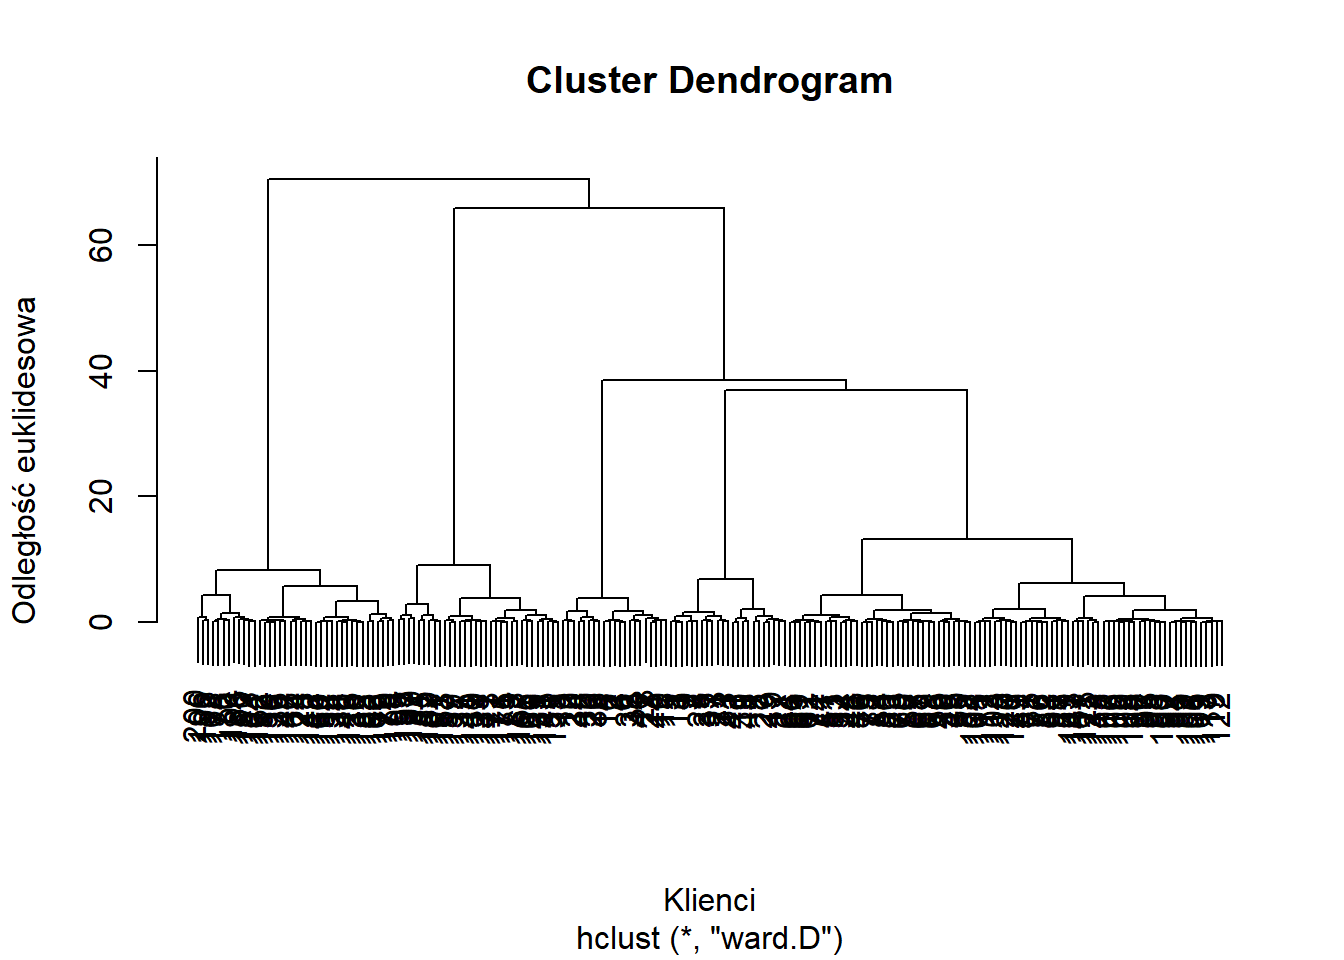
\includegraphics{Wawrowski_ADR_files/figure-latex/unnamed-chunk-38-1.pdf}

W ten sposób zostało zidentyfikowanych 22 obserwacji odstających. Korzystając z odległości Cooka wyeliminujemy obserwacje odstające ze zbioru:

\begin{Shaded}
\begin{Highlighting}[]
\NormalTok{outliers <-}\StringTok{ }\NormalTok{cook}\OperatorTok{$}\NormalTok{outliers}\OperatorTok{$}\NormalTok{observation}

\NormalTok{pracownicy_out <-}\StringTok{ }\NormalTok{pracownicy2[}\OperatorTok{-}\NormalTok{outliers,]}

\NormalTok{wybrany_model_out <-}\StringTok{ }\KeywordTok{lm}\NormalTok{(bwynagrodzenie }\OperatorTok{~}\StringTok{ }\NormalTok{pwynagrodzenie }\OperatorTok{+}\StringTok{ }\NormalTok{kat_pracownika }\OperatorTok{+}\StringTok{ }\NormalTok{doswiadczenie }\OperatorTok{+}\StringTok{ }\NormalTok{staz }\OperatorTok{+}\StringTok{ }\NormalTok{plec }\OperatorTok{+}\StringTok{ }\NormalTok{edukacja, }
                        \DataTypeTok{data =}\NormalTok{ pracownicy_out)}
\KeywordTok{summary}\NormalTok{(wybrany_model_out)}
\end{Highlighting}
\end{Shaded}

\begin{verbatim}
## 
## Call:
## lm(formula = bwynagrodzenie ~ pwynagrodzenie + kat_pracownika + 
##     doswiadczenie + staz + plec + edukacja, data = pracownicy_out)
## 
## Residuals:
##      Min       1Q   Median       3Q      Max 
## -12591.2  -2696.4   -564.8   2263.0  14704.1 
## 
## Coefficients:
##                   Estimate Std. Error t value Pr(>|t|)    
## (Intercept)     -3756.8288  2381.5361  -1.577 0.115420    
## pwynagrodzenie      1.3696     0.0676  20.260  < 2e-16 ***
## kat_pracownika2  6480.6971  1049.9539   6.172 1.56e-09 ***
## kat_pracownika3  9791.5000  1059.4980   9.242  < 2e-16 ***
## doswiadczenie     -18.5808     2.3229  -7.999 1.17e-14 ***
## staz              116.3809    20.9704   5.550 5.01e-08 ***
## plec1           -1616.6030   505.1391  -3.200 0.001475 ** 
## edukacja          397.7652   105.8146   3.759 0.000194 ***
## ---
## Signif. codes:  0 '***' 0.001 '**' 0.01 '*' 0.05 '.' 0.1 ' ' 1
## 
## Residual standard error: 4271 on 430 degrees of freedom
## Multiple R-squared:  0.894,  Adjusted R-squared:  0.8923 
## F-statistic: 518.3 on 7 and 430 DF,  p-value: < 2.2e-16
\end{verbatim}

Model dopasowany na takim zbiorze charakteryzuje się dużo mniejszym błędem standardowym oraz wyższym współczynnikiem \(R^2\) w porównaniu do poprzedniego. Sprawdźmy w takim razie normalność reszt.

\begin{Shaded}
\begin{Highlighting}[]
\KeywordTok{ols_plot_resid_qq}\NormalTok{(wybrany_model_out)}
\end{Highlighting}
\end{Shaded}

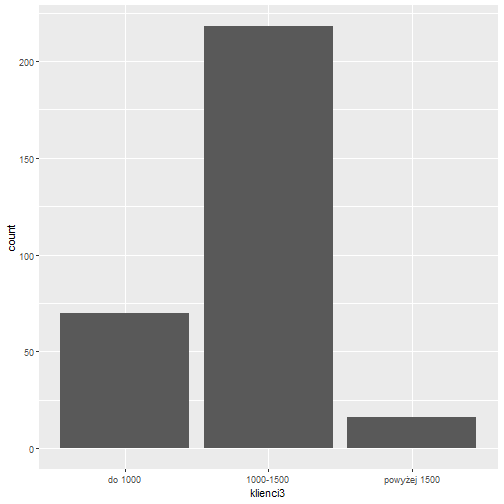
\includegraphics{Wawrowski_ADR_files/figure-latex/unnamed-chunk-40-1.pdf}

Wykres kwantyl-kwantyl wygląda już dużo lepiej i w zasadzie nie obserwuje tu się dużych odstępstw od rozkładu normalnego. Przeprowadźmy jeszcze odpowiednie testy statystyczne.

\begin{Shaded}
\begin{Highlighting}[]
\KeywordTok{ols_test_normality}\NormalTok{(wybrany_model_out)}
\end{Highlighting}
\end{Shaded}

\begin{verbatim}
## -----------------------------------------------
##        Test             Statistic       pvalue  
## -----------------------------------------------
## Shapiro-Wilk              0.9696         0.0000 
## Kolmogorov-Smirnov        0.0667         0.0405 
## Cramer-von Mises         38.1644         0.0001 
## Anderson-Darling          3.5421         0.0000 
## -----------------------------------------------
\end{verbatim}

Tylko test Kołmogorova-Smirnova na poziomie istotności \(\alpha=0,01\) wskazał na brak podstaw do odrzucenia hipotezy zerowej.

\hypertarget{zadanie-1}{%
\subsection{Zadanie}\label{zadanie-1}}

Na podstawie zbioru dotyczącego \href{data/startups.xlsx}{50 startupów} określ jakie czynniki wpływają na przychód startupów.

\begin{Shaded}
\begin{Highlighting}[]
\NormalTok{startupy <-}\StringTok{ }\KeywordTok{read_xlsx}\NormalTok{(}\StringTok{"data/startups.xlsx"}\NormalTok{)}

\NormalTok{startupy <-}\StringTok{ }\NormalTok{janitor}\OperatorTok{::}\KeywordTok{clean_names}\NormalTok{(startupy)}

\KeywordTok{summary}\NormalTok{(startupy)}
\end{Highlighting}
\end{Shaded}

\begin{verbatim}
##    r_d_spend      administration   marketing_spend     state          
##  Min.   :     0   Min.   : 51283   Min.   :     0   Length:50         
##  1st Qu.: 39936   1st Qu.:103731   1st Qu.:129300   Class :character  
##  Median : 73051   Median :122700   Median :212716   Mode  :character  
##  Mean   : 73722   Mean   :121345   Mean   :211025                     
##  3rd Qu.:101603   3rd Qu.:144842   3rd Qu.:299469                     
##  Max.   :165349   Max.   :182646   Max.   :471784                     
##      profit      
##  Min.   : 14681  
##  1st Qu.: 90139  
##  Median :107978  
##  Mean   :112013  
##  3rd Qu.:139766  
##  Max.   :192262
\end{verbatim}

\hypertarget{grupowanie}{%
\chapter{Grupowanie}\label{grupowanie}}

\href{presentations/05_grupowanie.html}{Prezentacja}

\hypertarget{wprowadzenie-3}{%
\section{Wprowadzenie}\label{wprowadzenie-3}}

Grupowanie polega na przypisanie obiektów do określonych grup/klastrów/skupień/segmentów, w których znajdą się jednostki najbardziej do siebie podobne, a powstałe grupy będą się między sobą różnić. Całe utrudnienie polega na tym, że nie wiemy ile tych grup ma powstać.

\hypertarget{metoda-k-srednich}{%
\section{Metoda k-średnich}\label{metoda-k-srednich}}

Najpopularniejszą metodą grupowania jest metoda k-średnich. Do jej zalet należy zaliczyć to, że dobrze działa zarówno na małych, jak i dużych zbiorach i jest bardzo efektywny - zwykle osiąga zbieżność w mniej niż 10 iteracjach. Z wad należy wskazać losowy wybór początkowych centrów skupień, co może skutkować nieprawidłowym przypisaniem obiektów do grup.

Algorytm postępowania jest następujący:

\begin{enumerate}
\def\labelenumi{\arabic{enumi}.}
\tightlist
\item
  Wskaż liczbę grup \(k\).
\item
  Wybierz dowolne \(k\) punktów jako centra grup.
\item
  Przypisz każdą z obserwacji do najbliższego centroidu.
\item
  Oblicz nowe centrum grupy.
\item
  Przypisz każdą z obserwacji do nowych centroidów. Jeśli któraś obserwacja zmieniła grupę - przejdź do kroku nr 4, a w przeciwnym przypadku zakończ algorytm.
\end{enumerate}

Wykorzystamy informacje ze zbioru zawierającego informacje o \href{data/klienci.csv}{klientach sklepu} i dokonamy grupowania tych klientów.

Opis zbioru:

\begin{itemize}
\tightlist
\item
  klientID - identyfikator klienta
\item
  plec - płeć
\item
  wiek - wiek
\item
  roczny\_dochod - roczny dochód wyrażony w tys. dolarów
\item
  wskaznik\_wydatkow - klasyfikacja sklepu od 1 do 100
\end{itemize}

Wczytujemy zbiór danych i sprawdzamy czy pomiędzy zmiennymi są widoczne jakieś zależności.

\begin{Shaded}
\begin{Highlighting}[]
\KeywordTok{library}\NormalTok{(tidyverse)}

\NormalTok{klienci <-}\StringTok{ }\KeywordTok{read.csv}\NormalTok{(}\StringTok{"data/klienci.csv"}\NormalTok{)}

\KeywordTok{ggplot}\NormalTok{(klienci, }\KeywordTok{aes}\NormalTok{(}\DataTypeTok{x=}\NormalTok{wiek, }\DataTypeTok{y=}\NormalTok{roczny_dochod)) }\OperatorTok{+}
\StringTok{  }\KeywordTok{geom_point}\NormalTok{()}
\end{Highlighting}
\end{Shaded}

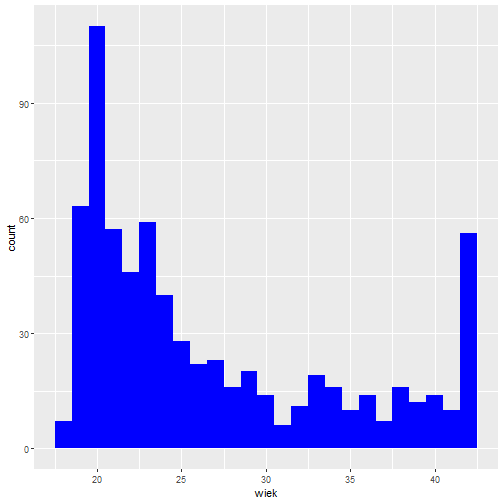
\includegraphics{Wawrowski_ADR_files/figure-latex/unnamed-chunk-43-1.pdf}

Pomiędzy wiekiem a rocznym dochodem nie widać zależności.

\begin{Shaded}
\begin{Highlighting}[]
\KeywordTok{ggplot}\NormalTok{(klienci, }\KeywordTok{aes}\NormalTok{(}\DataTypeTok{x=}\NormalTok{wiek, }\DataTypeTok{y=}\NormalTok{wskaznik_wydatkow)) }\OperatorTok{+}
\StringTok{  }\KeywordTok{geom_point}\NormalTok{()}
\end{Highlighting}
\end{Shaded}

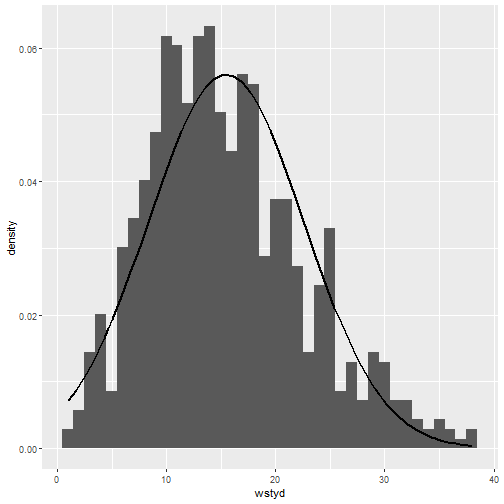
\includegraphics{Wawrowski_ADR_files/figure-latex/unnamed-chunk-44-1.pdf}

W przypadku wieku i wskaźnika wydatków moglibyśmy się pokusić o podział zbioru na dwie grupy za pomocą przekątnej.

\begin{Shaded}
\begin{Highlighting}[]
\KeywordTok{ggplot}\NormalTok{(klienci, }\KeywordTok{aes}\NormalTok{(}\DataTypeTok{x=}\NormalTok{wskaznik_wydatkow, }\DataTypeTok{y=}\NormalTok{roczny_dochod)) }\OperatorTok{+}
\StringTok{  }\KeywordTok{geom_point}\NormalTok{()}
\end{Highlighting}
\end{Shaded}

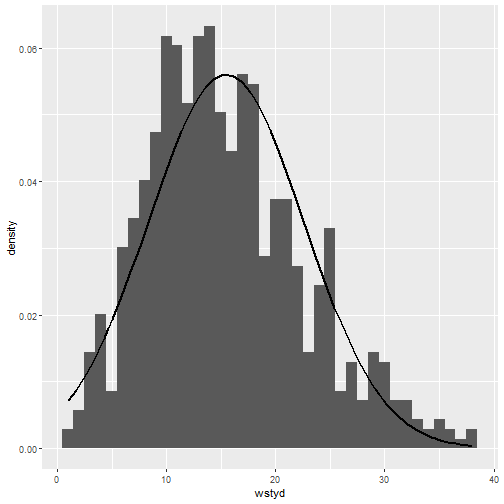
\includegraphics{Wawrowski_ADR_files/figure-latex/unnamed-chunk-45-1.pdf}

Po zestawieniu rocznego dochodu i wskaźnika wydatków wyłania się 5 potencjalnych grup, zatem te dwie cechy wykorzystamy do grupowania. Jednak przed zastosowaniem algorytmu musimy te dane przygotować normalizując zakres obu cech - w tym przypadku za pomocą standaryzacji.

\begin{Shaded}
\begin{Highlighting}[]
\NormalTok{klienci_z <-}\StringTok{ }\NormalTok{klienci }\OperatorTok
\StringTok{  }\KeywordTok{select}\NormalTok{(roczny_dochod, wskaznik_wydatkow) }\OperatorTok
\StringTok{  }\KeywordTok{scale}\NormalTok{()}

\KeywordTok{head}\NormalTok{(klienci_z)}
\end{Highlighting}
\end{Shaded}

\begin{verbatim}
##      roczny_dochod wskaznik_wydatkow
## [1,]     -1.734646        -0.4337131
## [2,]     -1.734646         1.1927111
## [3,]     -1.696572        -1.7116178
## [4,]     -1.696572         1.0378135
## [5,]     -1.658498        -0.3949887
## [6,]     -1.658498         0.9990891
\end{verbatim}

W przypadku, gdy podział na grupy nie jest tak oczywisty lub bierzemy pod uwagę więcej niż dwa kryteria to wówczas w wyznaczeniu optymalnej liczby skupień może pomóc wykres osypiska (ang. elbow method). Polega to na przeprowadzeniu grupowania (z wykorzystaniem funkcji \texttt{kmeans()}) dla różniej liczby grup i porównanie wariancji wewnątrz-grupowej. Dane do stworzenia wykresu osypiska możemy obliczyć w pętli:

\begin{Shaded}
\begin{Highlighting}[]
\NormalTok{zm_w_gr <-}\StringTok{ }\KeywordTok{numeric}\NormalTok{(}\DecValTok{15}\NormalTok{)}

\CommentTok{# wprowadzenie pętli}

\ControlFlowTok{for}\NormalTok{(i }\ControlFlowTok{in} \DecValTok{1}\OperatorTok{:}\KeywordTok{length}\NormalTok{(zm_w_gr)) \{}
  \KeywordTok{set.seed}\NormalTok{(}\DecValTok{14}\NormalTok{)}
\NormalTok{  gr <-}\StringTok{ }\KeywordTok{kmeans}\NormalTok{(klienci_z, }\DataTypeTok{centers =}\NormalTok{ i)}
\NormalTok{  zm_w_gr[i] <-}\StringTok{ }\NormalTok{gr}\OperatorTok{$}\NormalTok{tot.withinss}
\NormalTok{\}}

\KeywordTok{plot}\NormalTok{(}\DecValTok{1}\OperatorTok{:}\DecValTok{15}\NormalTok{, zm_w_gr, }\DataTypeTok{type=}\StringTok{"b"}\NormalTok{)}
\end{Highlighting}
\end{Shaded}

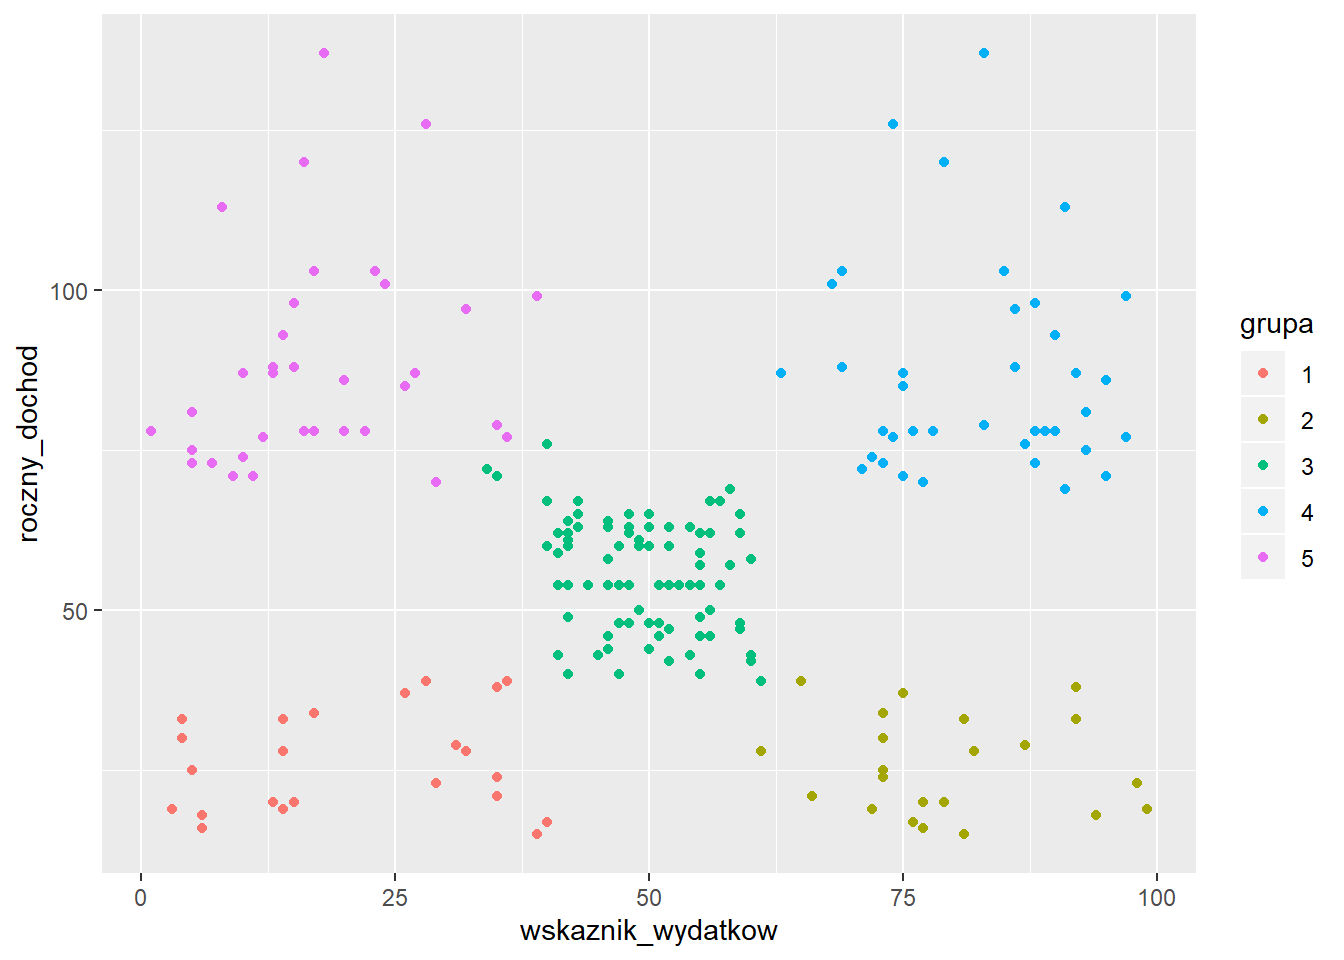
\includegraphics{Wawrowski_ADR_files/figure-latex/unnamed-chunk-47-1.pdf}

Wybieramy liczbę skupień po której nie następuje już gwałtowny spadek wartości wariancji wewnątrz-grupowej. Według tego kryterium powinniśmy wybrać wartość 6 zamiast 5. Sprawdźmy zatem jakie otrzymamy przyporządkowanie do grup. Następnie informację o tym przypisaniu umieszczamy w oryginalnym zbiorze danych i przedstawiamy na wykresie. W celu uzyskania powtarzalnych wyników zastosujemy stałe ziarno generatora.

\begin{Shaded}
\begin{Highlighting}[]
\KeywordTok{set.seed}\NormalTok{(}\DecValTok{12}\NormalTok{)}
\NormalTok{grupy <-}\StringTok{ }\KeywordTok{kmeans}\NormalTok{(}\DataTypeTok{x =}\NormalTok{ klienci_z, }\DataTypeTok{centers =} \DecValTok{5}\NormalTok{)}

\NormalTok{klienci}\OperatorTok{$}\NormalTok{grupa <-}\StringTok{ }\KeywordTok{as.factor}\NormalTok{(grupy}\OperatorTok{$}\NormalTok{cluster)}

\KeywordTok{ggplot}\NormalTok{(klienci, }\KeywordTok{aes}\NormalTok{(}\DataTypeTok{x=}\NormalTok{wskaznik_wydatkow, }
                    \DataTypeTok{y=}\NormalTok{roczny_dochod,}
                    \DataTypeTok{color=}\NormalTok{grupa)) }\OperatorTok{+}
\StringTok{  }\KeywordTok{geom_point}\NormalTok{()}
\end{Highlighting}
\end{Shaded}

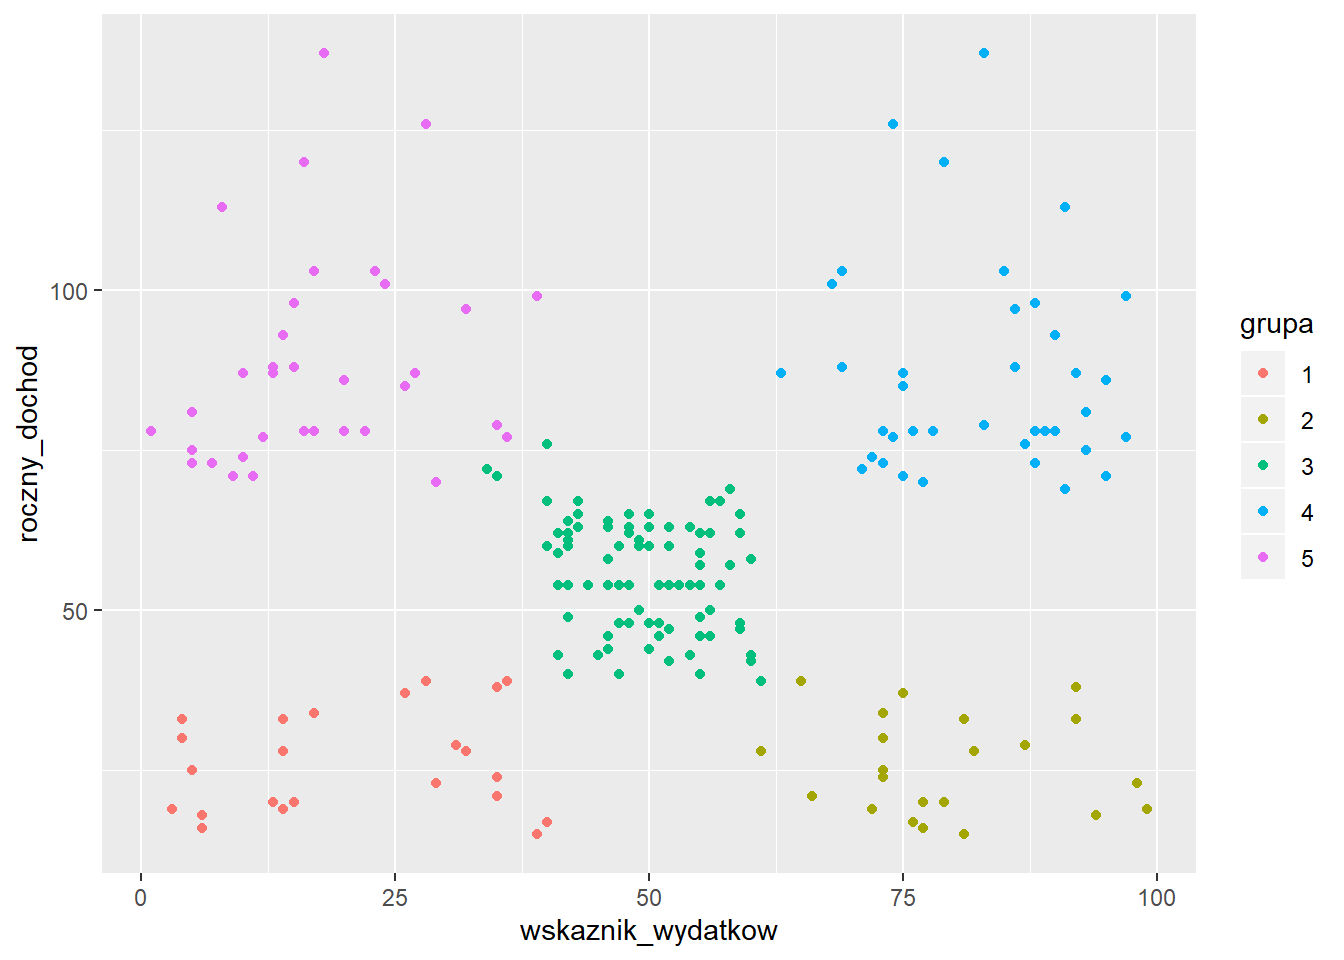
\includegraphics{Wawrowski_ADR_files/figure-latex/unnamed-chunk-48-1.pdf}

Jak zauważamy ten podział nie jest właściwy. Ze względu na losowy przydział centrów skupień na początku algorytmu istnieje spora szansa, że rozwiązanie nie będzie optymalne. Rozwiązaniem tego problemu jest użycie algorytmu kmeans++ do początkowego ustalenia centrów. Ta metoda jest zaimplementowana w pakiecie \texttt{ClusterR}. Ponadto jest tam także funkcja do ustalenia optymalnej liczby skupień na podstawie wykresu osypiska.

\begin{Shaded}
\begin{Highlighting}[]
\KeywordTok{library}\NormalTok{(ClusterR)}

\KeywordTok{Optimal_Clusters_KMeans}\NormalTok{(}\DataTypeTok{data =}\NormalTok{ klienci_z, }\DataTypeTok{max_clusters =} \DecValTok{15}\NormalTok{, }\DataTypeTok{criterion =} \StringTok{"WCSSE"}\NormalTok{)}
\end{Highlighting}
\end{Shaded}

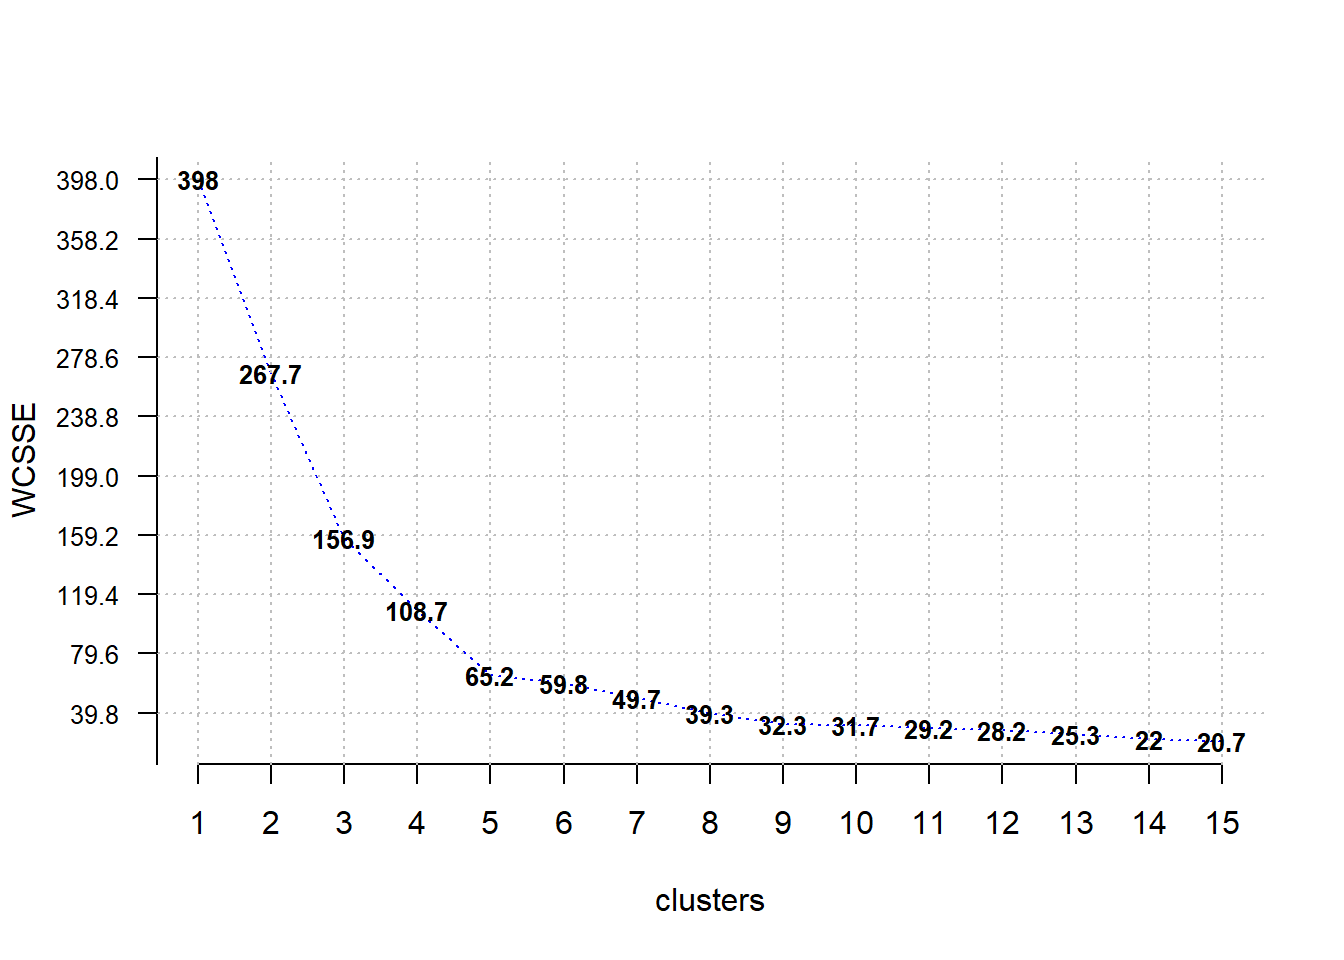
\includegraphics{Wawrowski_ADR_files/figure-latex/unnamed-chunk-49-1.pdf}

\begin{verbatim}
##  [1] 398.00000 267.67171 156.91549 108.68209  65.24057  59.83221  49.72816
##  [8]  39.31585  32.33261  31.70877  29.24003  28.18491  25.34096  22.01873
## [15]  20.67234
## attr(,"class")
## [1] "k-means clustering"
\end{verbatim}

Wybieramy liczbę skupień po której nie następuje już gwałtowny spadek wartości wariancji wewnątrz-grupowej. W analizowanym przypadku będzie to 5 grup. Następnie korzystamy z funkcji \texttt{KMeans\_rcpp} do wyznaczenia przynależności do grup. Ta funkcja domyślnie korzysta z algorytmu kmeans++, zatem nie ma niebezpieczeństwa, że uzyskamy niewłaściwe przyporządkowanie.

\begin{Shaded}
\begin{Highlighting}[]
\NormalTok{grupy2 <-}\StringTok{ }\KeywordTok{KMeans_rcpp}\NormalTok{(}\DataTypeTok{data =}\NormalTok{ klienci_z, }\DataTypeTok{clusters =} \DecValTok{5}\NormalTok{)}

\NormalTok{klienci}\OperatorTok{$}\NormalTok{grupa2 <-}\StringTok{ }\KeywordTok{as.factor}\NormalTok{(grupy2}\OperatorTok{$}\NormalTok{clusters)}

\KeywordTok{ggplot}\NormalTok{(klienci, }\KeywordTok{aes}\NormalTok{(}\DataTypeTok{x=}\NormalTok{wskaznik_wydatkow, }
                    \DataTypeTok{y=}\NormalTok{roczny_dochod,}
                    \DataTypeTok{color=}\NormalTok{grupa2)) }\OperatorTok{+}
\StringTok{  }\KeywordTok{geom_point}\NormalTok{()}
\end{Highlighting}
\end{Shaded}

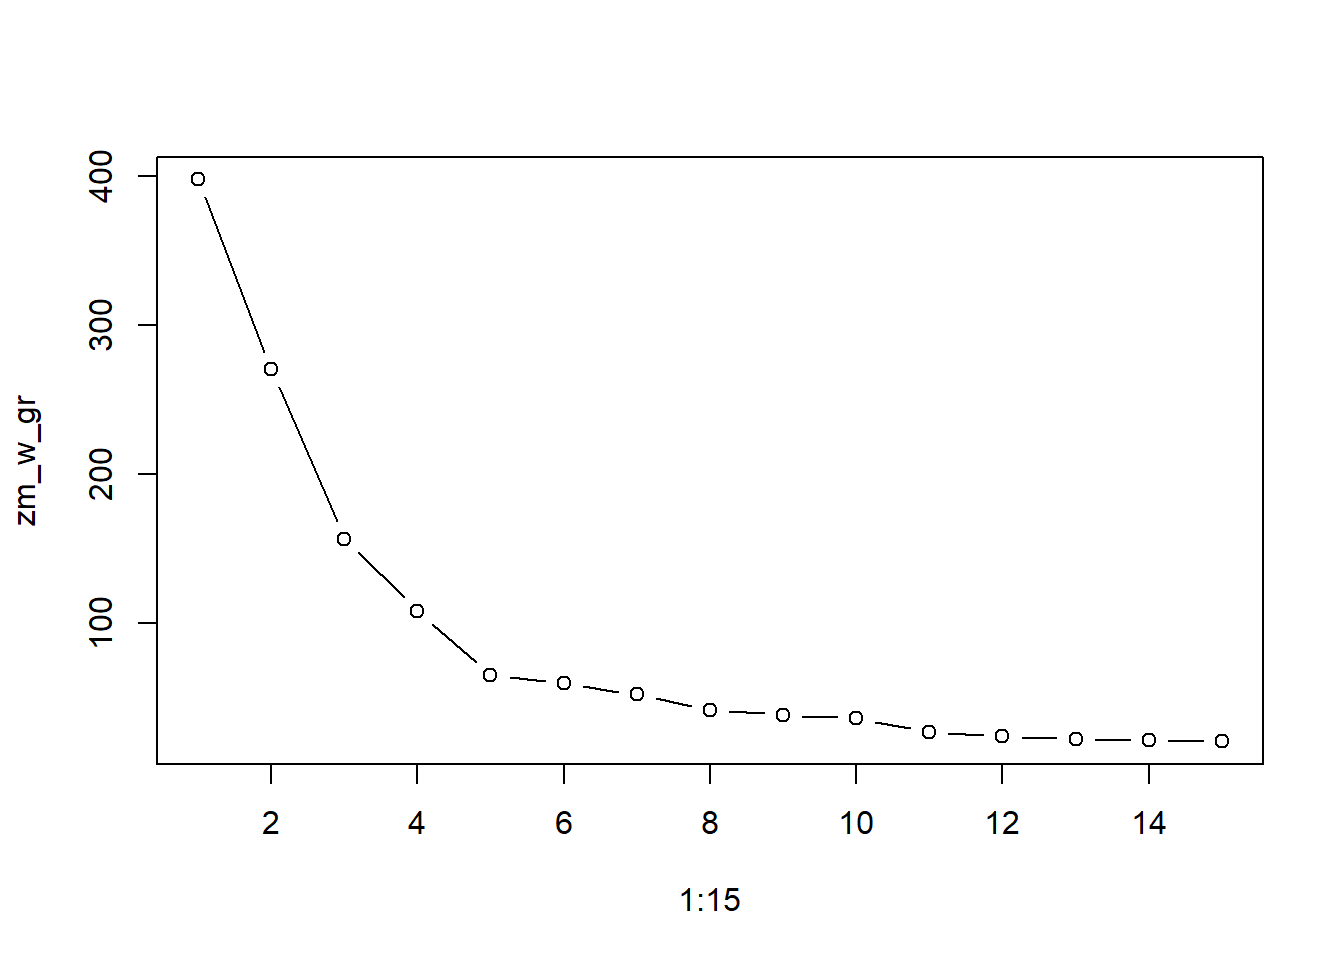
\includegraphics{Wawrowski_ADR_files/figure-latex/unnamed-chunk-50-1.pdf}

Ostatnim etapem analizy jest odpowiednia charakterystyka uzyskanych klastrów - najczęściej wyznacza się średnie wartości cech w ramach każdej grupy.

\begin{Shaded}
\begin{Highlighting}[]
\NormalTok{klienci }\OperatorTok
\StringTok{  }\KeywordTok{select}\NormalTok{(}\OperatorTok{-}\NormalTok{klientID, }\OperatorTok{-}\NormalTok{plec, }\OperatorTok{-}\NormalTok{grupa) }\OperatorTok
\StringTok{  }\KeywordTok{group_by}\NormalTok{(grupa2) }\OperatorTok
\StringTok{  }\KeywordTok{summarise_all}\NormalTok{(}\DataTypeTok{.funs =} \StringTok{"mean"}\NormalTok{)}
\end{Highlighting}
\end{Shaded}

\begin{verbatim}
## # A tibble: 5 x 4
##   grupa2  wiek roczny_dochod wskaznik_wydatkow
##   <fct>  <dbl>         <dbl>             <dbl>
## 1 1       25.3          25.7              79.4
## 2 2       45.2          26.3              20.9
## 3 3       41.1          88.2              17.1
## 4 4       32.7          86.5              82.1
## 5 5       42.7          55.3              49.5
\end{verbatim}

W grupie pierwszej znalazły się osoby z niskimi dochodami i wysokim wskaźnikiem wydatków. Grupa druga to klienci o niskich dochodach i wydatkach - ich przeciwieństwem jest grupa 4. W grupie 3 są osoby z wysokimi dochodami, ale niskimi wydatkami. Grupa 5 to z kolei średniacy - klienci o średnich dochodach i wydatkach.

\hypertarget{metoda-hierarchiczna}{%
\section{Metoda hierarchiczna}\label{metoda-hierarchiczna}}

Alternatywną metodą grupowania jest metoda hierarchiczna. Do jej zalet zaliczymy prosty sposób ustalenia liczby grup oraz praktyczny sposób wizualizacji. Niestety nie jest to metoda odpowiednia dla dużych zbiorów danych.

Algorytm postępowania:

\begin{enumerate}
\def\labelenumi{\arabic{enumi}.}
\tightlist
\item
  Każda obserwacji stanowi jedną z \(N\) pojedynczych grup.
\item
  Na podstawie macierzy odległości połącz dwie najbliżej leżące obserwacje w jedną grupę (\(N-1\) grup).
\item
  Połącz dwa najbliżej siebie leżące grupy w jedną (\(N-2\) grup).
\item
  Powtórz krok nr 3, aż do uzyskania jednej grupy.
\end{enumerate}

Dla tych samych danych przeprowadzimy grupowanie, ale tym razem metodą hierarchiczną. W metodzie hierarchicznej bazuje się na macierzy odległości pomiędzy obserwacjami. Można zastosować wiele miar odległości, ale najczęściej wykorzystywana jest odległość euklidesowa. Druga zmienna, na którą mamy wpływ to metoda łączenia skupień - w tym przypadku najlepsze rezultaty daje metoda Warda. Z kolei wyniki grupowania metodą hierarchiczną są prezentowane na dendrogramie.

\begin{Shaded}
\begin{Highlighting}[]
\NormalTok{macierz_odl <-}\StringTok{ }\KeywordTok{dist}\NormalTok{(klienci_z)}

\NormalTok{dendrogram <-}\StringTok{ }\KeywordTok{hclust}\NormalTok{(macierz_odl, }\DataTypeTok{method =} \StringTok{"ward.D"}\NormalTok{)}

\KeywordTok{plot}\NormalTok{(dendrogram, }\DataTypeTok{xlab=}\StringTok{"Klienci"}\NormalTok{, }\DataTypeTok{ylab=}\StringTok{"Odległość euklidesowa"}\NormalTok{)}
\end{Highlighting}
\end{Shaded}

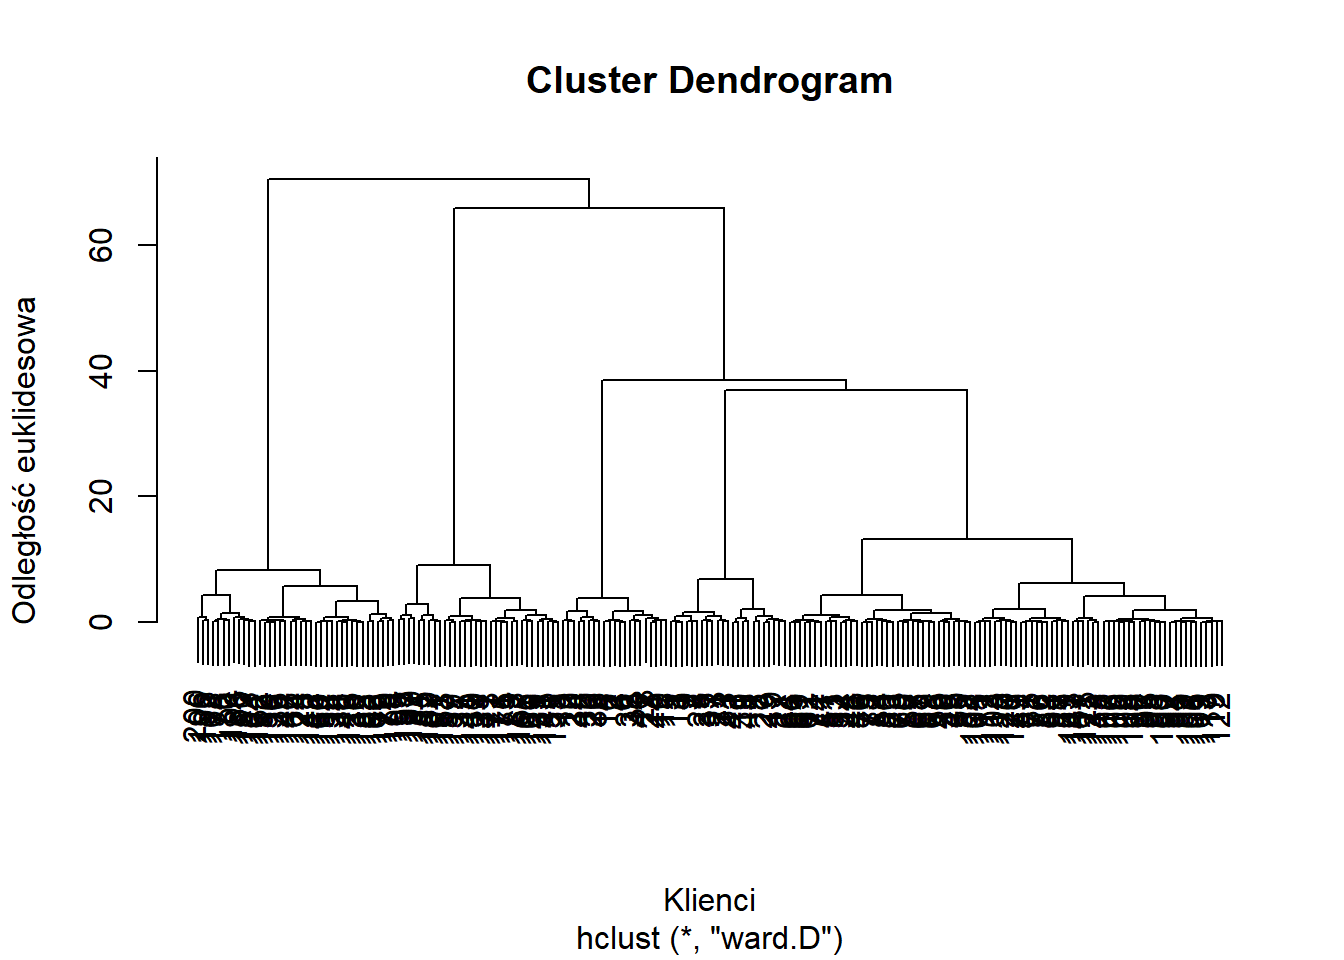
\includegraphics{Wawrowski_ADR_files/figure-latex/unnamed-chunk-52-1.pdf}

Na podstawie dendrogramu identyfikujemy największe różnice odległości opisane na osi Y. Także w tym przypadku identyfikujemy 5 grup. Istnieje także wiele kryteriów, które mają na celu wyznaczyć optymalną liczbę grup - link.

\begin{Shaded}
\begin{Highlighting}[]
\KeywordTok{plot}\NormalTok{(dendrogram, }\DataTypeTok{xlab=}\StringTok{"Klienci"}\NormalTok{, }\DataTypeTok{ylab=}\StringTok{"Odległość euklidesowa"}\NormalTok{)}
\KeywordTok{rect.hclust}\NormalTok{(dendrogram, }\DataTypeTok{k=}\DecValTok{5}\NormalTok{, }\DataTypeTok{border=}\StringTok{"red"}\NormalTok{)}
\end{Highlighting}
\end{Shaded}

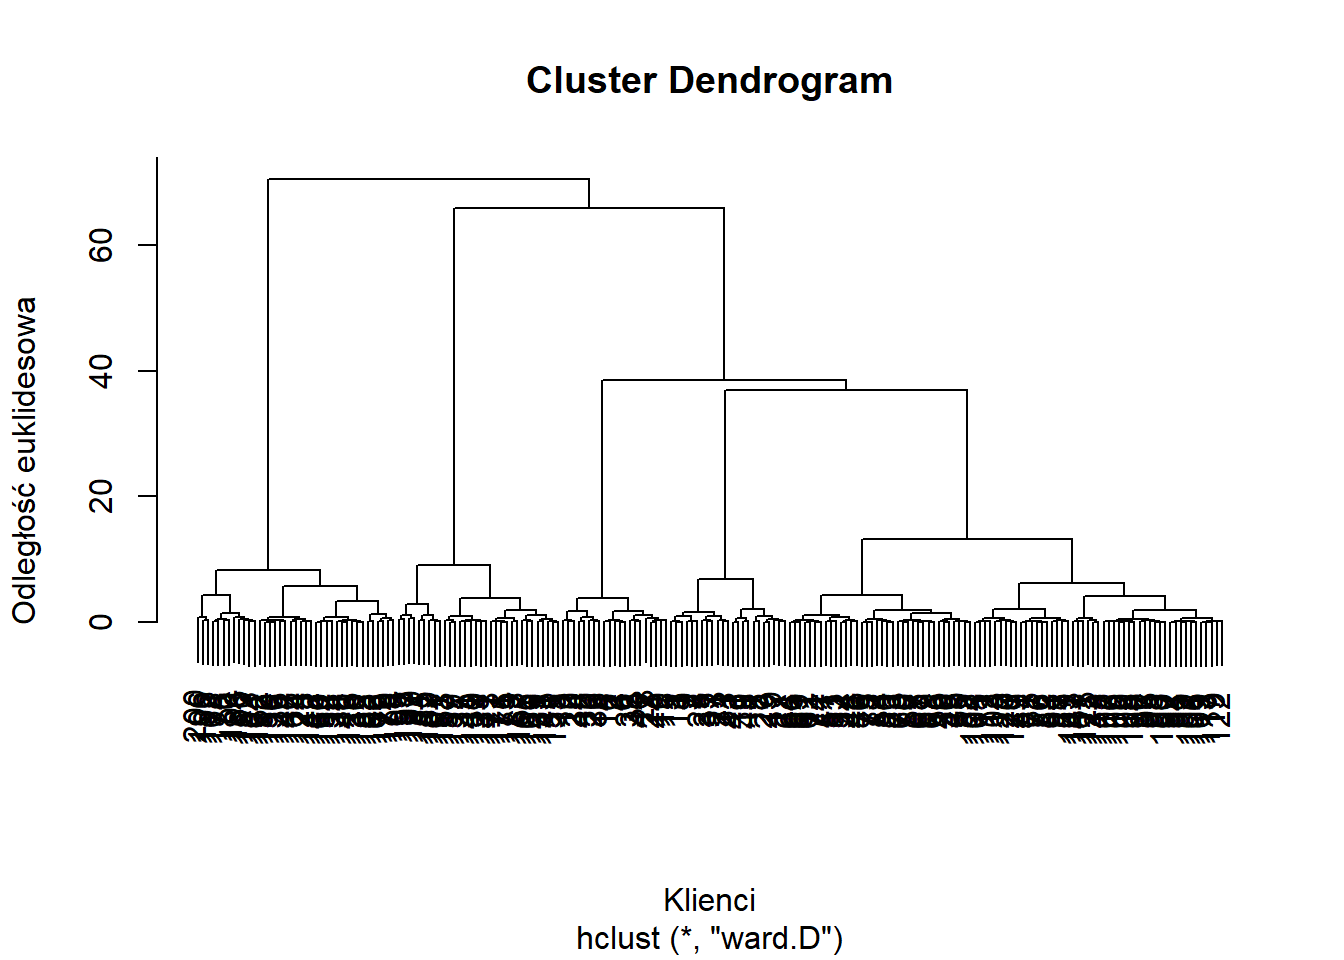
\includegraphics{Wawrowski_ADR_files/figure-latex/unnamed-chunk-53-1.pdf}

Następnie dopisujemy do oryginalnego zbioru danych etykiety utworzonych grup.

\begin{Shaded}
\begin{Highlighting}[]
\NormalTok{grupy_dendro <-}\StringTok{ }\KeywordTok{cutree}\NormalTok{(dendrogram, }\DecValTok{5}\NormalTok{)}

\NormalTok{klienci}\OperatorTok{$}\NormalTok{grupa3 <-}\StringTok{ }\KeywordTok{as.factor}\NormalTok{(grupy_dendro)}

\KeywordTok{ggplot}\NormalTok{(klienci, }\KeywordTok{aes}\NormalTok{(}\DataTypeTok{x=}\NormalTok{wskaznik_wydatkow, }
                    \DataTypeTok{y=}\NormalTok{roczny_dochod,}
                    \DataTypeTok{color=}\NormalTok{grupa3)) }\OperatorTok{+}
\StringTok{  }\KeywordTok{geom_point}\NormalTok{()}
\end{Highlighting}
\end{Shaded}

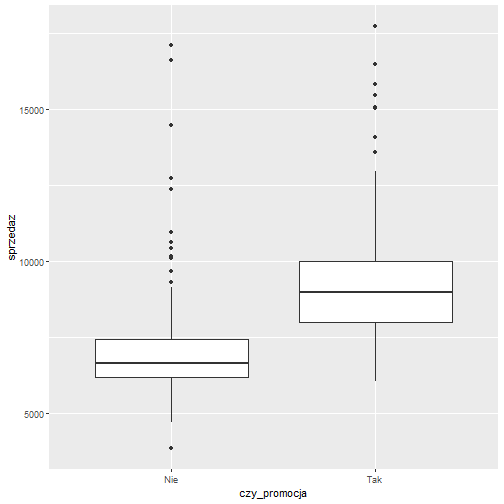
\includegraphics{Wawrowski_ADR_files/figure-latex/unnamed-chunk-54-1.pdf}

Uzyskane wyniki są bardzo zbliżone do tych otrzymanych za pomocą algorytmu k-średnich.

\begin{Shaded}
\begin{Highlighting}[]
\NormalTok{klienci }\OperatorTok
\StringTok{  }\KeywordTok{select}\NormalTok{(}\OperatorTok{-}\NormalTok{klientID, }\OperatorTok{-}\NormalTok{plec, }\OperatorTok{-}\NormalTok{grupa, }\OperatorTok{-}\NormalTok{grupa2) }\OperatorTok
\StringTok{  }\KeywordTok{group_by}\NormalTok{(grupa3) }\OperatorTok
\StringTok{  }\KeywordTok{summarise_all}\NormalTok{(}\DataTypeTok{.funs =} \StringTok{"mean"}\NormalTok{)}
\end{Highlighting}
\end{Shaded}

\begin{verbatim}
## # A tibble: 5 x 4
##   grupa3  wiek roczny_dochod wskaznik_wydatkow
##   <fct>  <dbl>         <dbl>             <dbl>
## 1 1       45.2          26.3              20.9
## 2 2       25.3          25.1              80.0
## 3 3       42.5          55.8              49.1
## 4 4       32.7          86.5              82.1
## 5 5       41            89.4              15.6
\end{verbatim}

Metoda hierarchiczna zastosowała inną numerację grup. Liczebności tych grup nieznacznie się różnią, ale charakterystyki wewnątrz grupowe są bardzo podobne do tych określonych na podstawie metody k-średnich.

Tworząc tabelę krzyżową możemy zobaczyć, że tylko 4 obserwacje zmieniły przypisanie do grup.

\begin{Shaded}
\begin{Highlighting}[]
\KeywordTok{table}\NormalTok{(klienci}\OperatorTok{$}\NormalTok{grupa2, klienci}\OperatorTok{$}\NormalTok{grupa3)}
\end{Highlighting}
\end{Shaded}

\begin{verbatim}
##    
##      1  2  3  4  5
##   1  0 21  1  0  0
##   2 23  0  0  0  0
##   3  0  0  3  0 32
##   4  0  0  0 39  0
##   5  0  0 81  0  0
\end{verbatim}

Porównajmy jeszcze wyniki działania tych dwóch metod na wykresach:

\begin{Shaded}
\begin{Highlighting}[]
\NormalTok{klienci }\OperatorTok
\StringTok{  }\KeywordTok{select}\NormalTok{(roczny_dochod, wskaznik_wydatkow, grupa2, grupa3) }\OperatorTok
\StringTok{  }\KeywordTok{gather}\NormalTok{(metoda, grupa, }\OperatorTok{-}\NormalTok{roczny_dochod, }\OperatorTok{-}\NormalTok{wskaznik_wydatkow) }\OperatorTok
\StringTok{  }\KeywordTok{ggplot}\NormalTok{(}\KeywordTok{aes}\NormalTok{(}\DataTypeTok{x=}\NormalTok{wskaznik_wydatkow, }\DataTypeTok{y=}\NormalTok{roczny_dochod)) }\OperatorTok{+}
\StringTok{  }\KeywordTok{geom_point}\NormalTok{(}\KeywordTok{aes}\NormalTok{(}\DataTypeTok{color=}\NormalTok{grupa)) }\OperatorTok{+}
\StringTok{  }\KeywordTok{facet_wrap}\NormalTok{(}\OperatorTok{~}\StringTok{ }\NormalTok{metoda)}
\end{Highlighting}
\end{Shaded}

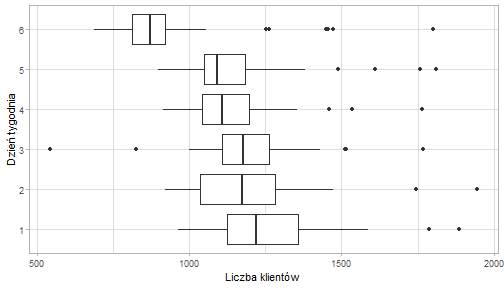
\includegraphics{Wawrowski_ADR_files/figure-latex/unnamed-chunk-57-1.pdf}

Problematyczne obserwacje pochodziły z grupy klientów o przeciętnych dochodach oraz wydatkach.

\hypertarget{zadania}{%
\subsection{Zadania}\label{zadania}}

\begin{enumerate}
\def\labelenumi{\arabic{enumi}.}
\item
  Dokonaj grupowania danych dotyczących \href{data/auta.csv}{32 samochodów} według następujących zmiennych: pojemność, przebieg, lata oraz cena.
\item
  Rozpoznawanie czynności na podstawie danych z przyspieszeniomierza w telefonie: \href{http://archive.ics.uci.edu/ml/datasets/User+Identification+From+Walking+Activity\#}{User Identification From Walking Activity Data Set}
\end{enumerate}

\hypertarget{klasyfikacja}{%
\chapter{Klasyfikacja}\label{klasyfikacja}}

\href{http://www.r2d3.us/visual-intro-to-machine-learning-part-1/}{A visual introduction to machine learning}

\hypertarget{drzewa-klasyfikacyjne}{%
\section{Drzewa klasyfikacyjne}\label{drzewa-klasyfikacyjne}}

Zalety:

\begin{itemize}
\tightlist
\item
  łatwa interpretacja
\item
  nie trzeba normalizować cech
\item
  rozwiązuje problemy liniowe i nieliniowe
\end{itemize}

Wady:

\begin{itemize}
\tightlist
\item
  mała efektywność przy małych zbiorach danych
\item
  łatwo można przeuczyć
\end{itemize}

\hypertarget{knn}{%
\section{KNN}\label{knn}}

Algorytm:

\begin{enumerate}
\def\labelenumi{\arabic{enumi}.}
\tightlist
\item
  Określ liczbę sąsiadów - \(K\)
\item
  Wyznacz \(K\) sąsiadów dla nowego punktu na podstawie wybranej odległości
\item
  Oblicz liczbę sąsiadów, w każdej z grup
\item
  Przypisz nową obserwację do grupy, w której ma więcej najbliższych sąsiadów
\end{enumerate}

Zalety:

\begin{itemize}
\tightlist
\item
  łatwa interpretacja
\item
  szybki i efektywny
\end{itemize}

Wady:

\begin{itemize}
\tightlist
\item
  trzeba określić liczbę sąsiadów
\end{itemize}

\hypertarget{zadanie-2}{%
\subsection{Zadanie}\label{zadanie-2}}

Zbuduj model klasyfikacyjny dla zbioru \href{data/Social_Network_Ads.csv}{danych} dotyczących cech internautów oraz informacji czy zamówili reklamowany produkt czy nie.

Przeprowadź imputację braków danych dla zbioru \href{data/pracownicy.RData}{pracowników}.

\hypertarget{materiay-z-zajec}{%
\chapter{Materiały z zajęć}\label{materiay-z-zajec}}

\hypertarget{section}{%
\section{28.10.2018}\label{section}}

\href{res/skrypt20181028.R}{Wprowadzenie do R}

\href{res/analiza20181028.R}{Analiza sejmików}

\hypertarget{section-1}{%
\section{18.11.2018}\label{section-1}}

\href{https://departmentofstatisticspue.github.io/statystyka-opisowa/analiza-struktury.html}{Analiza struktury}

\href{data/rossmann.xlsx}{Rossmann}

\href{res/zajecia20181118.R}{Analiza struktury w R}

\hypertarget{section-2}{%
\section{16.12.2018}\label{section-2}}

\href{prezentacje/03.html}{Prezentacja}

\href{data/Salary_Data.csv}{Pracownicy}

\href{res/korelacje20181216.R}{Korelacja w R}

\href{res/regresja20181216.Rmd}{Regresja w R}

\hypertarget{section-3}{%
\section{26.01.2019}\label{section-3}}

\href{data/salary.xlsx}{Pensja i doświaczenie}

\href{data/pracownicy.xlsx}{Pracownicy}

Opis zbioru:

\begin{itemize}
\tightlist
\item
  id - kod pracownika
\item
  plec - płeć pracownika (0 - mężczyzna, 1 - kobieta)
\item
  data\_urodz - data urodzenia
\item
  edukacja - wykształcenie (w latach nauki)
\item
  kat\_pracownika - grupa pracownicza (1 - ochroniarz, 2 - urzędnik, 3 - menedżer)
\item
  bwynagrodzenie - bieżące wynagrodzenie
\item
  pwynagrodzenie - początkowe wynagrodzenie
\item
  staz - staż pracy (w miesiącach)
\item
  doswiadczenie - poprzednie zatrudnienie (w miesiącach)
\item
  zwiazki - przynależność do związków zawodowych (0 - nie, 1 - tak)
\item
  wiek - wiek (w latach)
\end{itemize}

\href{res/regresja20190126.R}{Regresja w R}


\end{document}
